\PassOptionsToPackage{dvipsnames}{xcolor}
\documentclass[a4paper,11pt]{article}

\usepackage{jheppub}
\usepackage{amsmath,amssymb,amsthm,mathtools}
\usepackage{bm}
\usepackage{booktabs,array}
\usepackage{float}
\usepackage{enumitem}
\usepackage{microtype}
\usepackage{tikz}
\usetikzlibrary{calc,positioning}
\hypersetup{
  colorlinks=true,
  linkcolor=MidnightBlue,
  citecolor=MidnightBlue,
  urlcolor=MidnightBlue,
  pdftitle={Hidden Region Finder}
}

\newcommand{\x}{\boldsymbol{x}}
\newcommand{\s}{\boldsymbol{s}}
\newcommand{\K}{\mathcal K}
\newcommand{\HR}{\mathrm{HR}}
\newcommand{\SL}{\mathrm{SL}}
\newcommand{\Obs}{\mathrm{Obs}}
\newcommand{\FSL}{\mathcal F_{\rm SL}}
\newcommand{\SSL}{\mathcal S_{\rm SL}}
\newcommand{\FObs}{\mathcal F_{\rm Obs}}
\newcommand{\WSL}{W_{\rm SL}}
\newcommand{\WHR}{W_{\rm HR}}
\newcommand{\vHR}{\vec v_{\rm HR}}
\newcommand{\Rpos}{\mathbb R_{>0}}
\newcommand{\ideal}{\mathcal I}
\newcommand{\dd}{\mathrm d}
\newcommand{\SLcolour}[1]{{\color{red}#1}}
\newcommand{\HRcolour}[1]{{\color{blue}#1}}
\newcommand{\Othercolour}[1]{{\color{black}#1}}

\tikzset{
 hrf internal/.style={thick},
 hrf contracted/.style={thick,densely dashed,red},
 hrf vertex/.style={circle,fill=black,draw=black,minimum size=3.2pt,
                    inner sep=0pt,outer sep=0pt},
 hrf edge label/.style={fill=white,inner sep=1pt,font=\scriptsize},
 hrf leg label/.style={font=\small}
}

\newtheorem{principle}{Principle}
\newtheorem{remark}{Remark}

\title{Hidden Region Finder}

% Replace the placeholders below with the author information.
% Use the same affiliation label for authors at the same institution.
%
% \author[a]{First Author}
% \author[b]{Second Author}
% \affiliation[a]{First institution, address, country}
% \affiliation[b]{Second institution, address, country}
% \emailAdd{first.author@example.org}
% \emailAdd{second.author@example.org}

\author{Einan Gardi}
\affiliation{Higgs Centre for Theoretical Physics, School of Physics and Astronomy,\\ The University of Edinburgh, Edinburgh EH9 3FD, United Kingdom}

\emailAdd{Einan.Gardi@ed.ac.uk}

\abstract{The Method of Regions is a systematic way to derive asymptotic
expansions of Feynman integrals.  For Euclidean integrals there is a
well-established algorithm that determines the complete set of regions from
the facets of a Newton polytope defined by the graph polynomials.  In many
physically relevant Minkowski limits this construction misses additional
contributions, known as hidden regions.  A hidden region arises when an
asymptotic scaling makes a set of monomials parametrically superleading, but
these enhanced monomials cancel collectively at a pinch singularity on the
contour of positive Schwinger parameters.  Their sum is thereby reduced to the
same order as terms which appeared subleading before the cancellation.

We present the Hidden Region Finder, a parameter-space algorithm that
identifies such pinch singularities and determines the associated hidden
regions and their scaling laws.

We explore massless four-, five- and six-point integrals in a variety of
wide-angle, collinear, double-collinear and Regge limits.  Across these
different expansions, hidden regions recur in the same small set of seed
topologies.  This exploratory study showcases the potential of the Hidden
Region Finder both to uncover missing contributions to asymptotic expansions
and to reveal topology-based relations between physically distinct
kinematic limits.}

\begin{document}
\maketitle
\flushbottom



\section{Introduction}


Hidden regions are contributions to asymptotic expansions that are invisible
to the ordinary Newton-polytope formulation of the Method of Regions because
nominally leading monomials cancel on a positive Landau pinch.  We introduce
the Hidden Region Finder (HRF), a parameter-space construction that determines
the cancellation locus, the superleading and obstruction polynomials, the
region scaling and the resolved leading Lee--Pomeransky polynomial.  It
handles general polynomial cancellation ideals, contraction-boundary
regions, asymptotic-order alignment and successive cancellation layers.  We
develop the construction for massless internal propagators, where the
Symanzik polynomials are linear in every individual Schwinger parameter.

Applications reveal a sparse topology-based organization that is not apparent
from individual region searches.  In the audited on-shell four-point sample
through four loops, every certified wide-angle or three-channel Regge hidden
region is associated with the three-loop Crown, either in the graph interior
or as a contraction minor; an exhaustive analysis of 16 mixed-sign four-loop
topologies without a Crown minor finds none.  These results support both the
Crown-minor and wide-angle-to-Regge conjectures in this sample.  In
addition, the five-loop SuperCrown supplies a positive contraction-minor test
beyond the four-loop audit.  In five-point scattering, the same two-loop
seed supports distinct HRs in a spacelike-collinear expansion and in a
composite multi-Regge limit with a soft central emission.  Complete edge-flow
tables and a light-cone pole-pinch audit determine the local Glauber modes and
make the momentum-space reconstruction mode complete; a vertex-corrected spacelike descendant also shows why
genuinely non-binomial cancellation factors are required.
At six points, asymptotic-order alignment exposes a common positive
cancellation hypersurface for NMRK with \(w=z\) and for the double
spacelike-collinear limit.  The two expansions share the same factorized
superleading support but resolve it at different cancellation depths, and
therefore have distinct region vectors.  Thus HRF is not only a region-finding
algorithm: it exposes seed topologies and relations between kinematic
expansions.
The Method of Regions (MoR) constructs the asymptotic expansion of a
multiscale Feynman integral as a sum of integrals associated with distinct
scalings of the integration variables.  Its geometric formulation in
parameter space maps every monomial of the Lee--Pomeransky polynomial to an
exponent point.  Lower facets of the resulting Newton polytope determine the
ordinary endpoint regions and their scaling vectors.

The Newton polytope retains the monomial exponents but not the information
carried by their coefficients.  In a physical Minkowski region, monomials of
opposite sign can cancel at positive values of the parameters.  If the
cancellation is reinforced by a Landau pinch, a set of monomials may be
individually more singular than the physical leading contribution while
their sum is suppressed.  The corresponding scaling is not a lower-facet
normal of the original polynomial and is therefore hidden from the ordinary
geometric construction.  We call it a \emph{hidden region} (HR).

A hidden region is specified by more than a scaling vector.  One must
identify the common positive cancellation locus, determine which monomials
form the superleading sector, resolve their cancellation against the
remaining Lee--Pomeransky polynomial, and verify that the resulting leading
integral is scaleful.  The Hidden Region Finder (HRF) is the systematic
parameter-space construction that performs these tasks.

The present paper concerns massless internal propagators only.  This is a
structural restriction, not a choice of examples: both Symanzik polynomials
are then multiaffine, or equivalently linear in every individual edge
parameter.  Internal masses add
\(\mathcal U\sum_e m_e^2x_e\) to \(\mathcal F\), which can generate
quadratic dependence on an individual \(x_e\).  Hidden regions in that more
general setting are important, but require a separate extension of the
construction and will not be treated here.

The presentation has two parts.  Part~I defines the construction without
reference to a particular graph.  Part~II develops the same ideas through a
sequence of massless examples.  Each example introduces one additional
phenomenon: a factorised cancellation with uniform scaling; an obstruction
that fixes a non-uniform scaling; non-binomial cancellation factors; and
finally composite limits for which preliminary asymptotic-order alignment
and, in some cases, more than one cancellation layer are required.  The
examples also reveal a recurring physical organisation: a special seed
topology can support different HRs in different kinematic expansions.

\section{Hidden Regions Finder: Principles}
\label{sec:principles}

\subsection{Parameter-space setup and definitions}
\label{sec:notation}

Consider a graph \(\mathcal G\) with \(N\) massless internal propagators and Lee--Pomeransky
(LP) polynomial
\begin{equation}
  \mathcal P(\x,\s)=\mathcal U(\x)+\mathcal F(\x;\s).
\end{equation}
The spanning-tree and spanning-2-forest formulae make the relevant structure
immediate.  For an \(L\)-loop graph, \(\mathcal U\) is homogeneous of degree
\(L\), while \(\mathcal F\) is homogeneous of degree \(L+1\) in the edge
parameters.  Each edge occurs at most once in every complementary
tree or 2-forest product.  Hence, for massless internal propagators, both
graph polynomials are linear in each individual \(x_e\).  This
multiaffinity is a standing assumption below.
Up to a normalisation which is irrelevant here, its integral has the form
\begin{equation}
 I_{\mathcal G}
 =
 \mathcal N_{\rm LP}
 \int_0^\infty
 \prod_{e=1}^{N}\frac{\dd x_e}{x_e}\,x_e^{\nu_e}\,
 \mathcal P(\x,\s)^{-D/2}.
\label{eq:LP}
\end{equation}
The \(N\) variables \(x_e\) are independent Lee--Pomeransky edge parameters,
each integrated over \((0,\infty)\).  In particular, there is no constraint
on \(\sum_e x_e\), or on the sum of any subset of the parameters.  We use
\(x_e\) rather than the conventional Feynman-parameter symbol \(\alpha_e\).

An optional, distinct projective representation can be obtained by
introducing one additional parameter \(x_0\) and the homogeneous polynomial
\begin{equation}
 \widehat{\mathcal P}(x_0,\x;\s)
 =\mathcal F(\x;\s)+x_0\mathcal U(\x).
\label{eq:homogenised-LP}
\end{equation}
There are then \(N+1\) parameters, and their common rescaling may be fixed by
inserting \(\delta(1-E(x_0,\x))\) for any positive degree-one homogeneous
function \(E\).  This homogenised embedding is distinct from the
non-projective LP integration space in \eqref{eq:LP} and is not assumed here.

Let \(\delta\to0^+\) define the kinematic expansion, and let \(\s\) denote a
set of real kinematic coordinates.  No sign convention is imposed on the
individual components of \(\s\); a physical domain \(\K\) is specified by
the appropriate inequalities among them.  This allows the same variables to
be retained across different physical regions, making changes of sign under
crossing or analytic continuation explicit.  A separate positive
parametrisation of a particular domain may be introduced locally as a
bookkeeping aid for proving inequalities or performing semialgebraic sign
tests, but neither the Newton-polytope construction nor the first-sheet pinch
condition requires it.  Retaining signed common variables also makes a
change in the existence of a cancellation directly visible in a factorised
superleading polynomial.  After expanding the kinematics, write
\begin{equation}
 \mathcal P(\x,\delta;\s)
 =
 \sum_i m_i,
 \qquad
 m_i\equiv
 c_i(\s)\,
 \delta^{a_i}\x^{\boldsymbol r_i},
 \qquad
 \x^{\boldsymbol r_i}
 =\prod_{e=1}^{N}x_e^{r_{i,e}}.
\label{eq:Pmonomials}
\end{equation}
Thus
\(\boldsymbol r_i=(r_{i,1},\ldots,r_{i,N})\) is the length-\(N\)
LP-parameter exponent vector of the monomial \(m_i\), while its augmented
length-\(N+1\) exponent point is
\begin{equation}
 \vec r_i=(\boldsymbol r_i;a_i)\in\mathbb R^{N+1}.
\end{equation}
No fixed sign of \(m_i\) on the whole physical domain is assumed.  Although
\(\delta^{a_i}\x^{\boldsymbol r_i}>0\) for \(\delta>0\) and \(\x>0\), the
coefficient \(c_i(\s)\) may vanish and change sign within or between the
domains under comparison.  The same qualification applies if several literal monomials have
been grouped into a kinematic coefficient or polynomial term.
A region vector is represented by an augmented normal whose last component
is normalised to one,
\begin{equation}
 \vec v_R=(\boldsymbol v_R;1),
 \qquad
 x_e\longmapsto \delta^{v_{R,e}}x_e,
\label{eq:regionvector}
\end{equation}
and the weight of a monomial is
\begin{equation}
 w_R(m_i)=\vec v_R\cdot\vec r_i
 =a_i+\boldsymbol v_R\cdot\boldsymbol r_i.
\label{eq:weight}
\end{equation}
The last component is always displayed when a vector is meant to be a
normal in augmented exponent space.  A list containing only the first \(N\)
entries is an LP-parameter scaling and not a fully normalised augmented
normal.

For a cancellation-free polynomial, the monomials of minimum weight form a
lower face of its Newton polytope.  A codimension-one lower face has an
inward-pointing normal whose last component is positive; after normalising
that component to one, the normal gives the corresponding facet-region
scaling.

\subsubsection{Positive pinches}
\label{sec:pinch}

The LP variables are integrated on the positive contour
\(\mathcal C_{\rm LP}=\mathbb R_{>0}^{N}\).  An interior first-sheet pinch of
a polynomial \(\mathcal Q(\x;\s)\) is therefore a solution
\begin{equation}
 \mathcal Q=0,
 \qquad
 \frac{\partial\mathcal Q}{\partial x_e}=0
 \quad(e=1,\ldots,N),
 \qquad
 \x\in\mathbb R_{>0}^{N},\quad \s\in\K.
\label{eq:positive-pinch}
\end{equation}
For a homogeneous polynomial, the derivative equations imply
\(\mathcal Q=0\) by Euler's identity.  On a contraction stratum the same
equations are imposed only on the active, nonzero parameters.

A cancellation in the positive orthant requires terms of both signs.
Consequently, every active derivative at an interior pinch must either vanish
identically or contain terms of both signs.  This elementary necessary
condition is useful as a rapid prefilter, but it neither identifies the
common pinch locus nor proves that a hidden region exists.  The defining
conditions below first use the scaling law to isolate \(\FSL\), and then
require a simultaneous positive solution of its derivative equations.

\subsubsection{Definition of a hidden region}
\label{sec:definition}

A HR is characterised by a superleading monomial support \(\SSL\), its
associated polynomial
\begin{equation}
 \FSL=\sum_{i\in\SSL}m_i,
\label{eq:FSLsupport}
\end{equation}
and a final scaling
\begin{equation}
 \vHR=(\boldsymbol v_{\HR};1)
\end{equation}
such that:
\begin{enumerate}[label=(\alph*)]
\item every monomial indexed by \(i\in\SSL\) has the same individual weight,
      \begin{equation}
        w_{\HR}(m_i)=\WSL,
        \qquad i\in\SSL;
      \label{eq:SLhomogeneity}
      \end{equation}
\item \(\FSL\) has a common first-sheet pinch in \(\K\),
      \begin{equation}
       \left.
       \frac{\partial\FSL}{\partial x_e}
       \right|_{\x>0,\,\s\in\K}=0
       \qquad\text{for every active }x_e;
      \label{eq:SLpinch}
      \end{equation}
\item the cancellation suppresses the sum of the superleading monomials to
      the first nonvanishing LP layer of weight \(\WHR\), with
      \begin{equation}
        \WHR>\WSL;
      \label{eq:gap}
      \end{equation}
\item after resolving the cancellation, the leading LP polynomial defines a
      scaleful lower-facet region.
\end{enumerate}
The gap \(\WHR-\WSL\) measures the depth of the cancellation.  It is a
physical output of the full problem and is not a freely chosen normalisation.

The superleading sector is not defined merely by mixed signs.  Mixed signs
are necessary for an interior pinch, but the simultaneous positive solution,
the hierarchy, and the final lower-facet condition are all essential.

\begin{principle}[Scaling precedes the positive pinch test]
The mixed-sign test is applied to derivatives of the starting polynomial
\(\mathcal F_\star\), but the simultaneous Landau equations are not.  The
weight homogeneity and separation conditions must first isolate the support
\(\SSL\).  The positive first-sheet equations are then imposed on the
resulting polynomial \(\FSL\).  Generically
\(\partial\mathcal F_\star/\partial x_e=0\) has no simultaneous positive
solution because \(\mathcal F_\star\) still contains the obstruction and
other terms excluded by the HR scaling.
\label{pr:scaling-before-pinch}
\end{principle}

\subsection{The core HRF construction}
\label{sec:ordinary}

The core construction receives a specified starting polynomial
\(\mathcal F_\star\) on a specified set of active LP parameters.  It has two
parts.  The first constructs and validates a decomposition into a
superleading cancellation sector and an obstruction.  The second determines
the scaling, resolves the complete LP polynomial and certifies the resulting
lower facet.  The choices of starting face and contraction stratum are outer
operations discussed only after this core construction is complete.
Part~I may use homogeneous-weight and strict-separation equations to decide
whether a proposed support defines a valid decomposition.  This provisional
selection is distinct from Part~II, which determines and certifies the
physical total region vector from the complete LP polynomial.

Before any LP-parameter scaling, expand
\begin{equation}
 \mathcal F(\x,\delta;\s)
 =
 \mathcal F_0(\x;\s)
 +\sum_{n>0}\delta^n\mathcal F_n(\x;\s).
\label{eq:Fexpansion}
\end{equation}
When the relevant superleading monomials are contained in
\(\mathcal F_0\), the cancellation analysis begins with
\(\mathcal F_\star=\mathcal F_0\).

\subsubsection{Part I: constructing and validating the decomposition}

The derivatives of \(\mathcal F_\star\) are inspected for primitive,
non-monomial polynomial factors \(f_j(\x,\s)\) which can vanish for
\(\x>0\) and \(\s\in\K\).  At fixed \(\s\in\K\), a necessary condition
for such a zero is that the nonzero coefficients of the LP-parameter
monomials are not all of the same sign.  A
monomial factor such as \(x_e\) is not a cancellation hypersurface in the
interior and is removed from the primitive factor.

Literal factorisation and kinematic-coefficient harvesting are the first,
inexpensive form of this derivative harvest.  They need not expose every
primitive normal polynomial: the derivatives may contain only invertible
linear combinations of the normals.  At this stage, however, the derivatives
are inspected rather than imposed.  In particular, one must not replace this
harvest by the ideal generated by all derivatives of \(\mathcal F_\star\).
When an obstruction is present, its derivatives need not vanish on the true
HR locus even though the derivatives of the subsequently selected
\(\FSL\) do.  Saturating that full gradient ideal would merely impose the
wrong equations more efficiently.  The harvest therefore retains candidate
factors and kinematic sectors without requiring any complete derivative to
vanish.

This inspection generates candidate cancellation structures; it is not a
Landau test on \(\mathcal F_\star\).  In particular, the full derivative
system of \(\mathcal F_\star\) is not required to have a positive solution at
this stage and generically does not.  A generator-based candidate support is
retained only if it admits a homogeneous-weight solution that strictly
separates \(\SSL\) from the obstruction and all other monomials.  At this
stage these linear conditions validate the candidate decomposition; they do
not yet determine the certified physical total vector.

\paragraph{Generators and the obstruction decomposition.}

Candidate generators are products of genuine cancellation polynomials,
\begin{equation}
 g_k=\prod_{f_j\in S_k}f_j,
\end{equation}
with at least two cancellation factors in the generator structures used by
HRF.  The factors, not monomial edge parameters, define the singular
hypersurfaces.  For a generator set \(G=\{g_1,\ldots,g_r\}\), define
\begin{equation}
 \mathcal I_{\rm canc}(G)
 =
 \langle g_1,\ldots,g_r\rangle.
\end{equation}
The HRF seeks a decomposition
\begin{equation}
 \mathcal F_\star=\FSL+\FObs,
 \qquad
 \FSL\in\mathcal I_{\rm canc}(G),
\label{eq:obstruction}
\end{equation}
or equivalently
\begin{equation}
 \FSL=\sum_kM_k(\x,\s)g_k.
\label{eq:idealpresentation}
\end{equation}
The polynomial \(\FObs\) is the obstruction: it prevents the full starting
polynomial from vanishing on the candidate cancellation locus but is to be
suppressed relative to the individual SL monomials by the HR scaling.

Different generator presentations can describe the same ideal and the same
pinch locus.  The presentation is a discovery device and does not label a
physical region.  Polynomial multipliers \(M_k\) in
\eqref{eq:idealpresentation} are allowed; a special factorised presentation
valid for one topology must not be promoted to a general rejection rule.

\paragraph{Positive-pinch validation.}

Only for the selected polynomial \(\FSL\) is the simultaneous first-sheet
pinch condition imposed.  When its derivative equations reduce to a set of
primitive cancellation factors, physical admissibility requires a common
positive zero at one and the same kinematic point:
\begin{equation}
 \exists\,(\x,\s)\in\Rpos^N\times\K:
 \qquad f_1(\x,\s)=\cdots=f_r(\x,\s)=0.
\label{eq:commonzero}
\end{equation}
Equivalently one solves \eqref{eq:SLpinch} directly.  The common locus,
rather than any one factor in isolation, encodes the pinch.  The elementary
mixed-sign condition can discard impossible ingredients, but it cannot
replace the scaling selection of \(\SSL\) or the subsequent simultaneous
positive solution.

If literal factorisation is insufficient at this candidate-specific stage,
one may complete the same calculation algebraically.  Let us define the
selected leading-sector gradient ideal \(\mathcal I_\nabla^{\rm SL}\) and
the localization element \(S\) by
\begin{equation}
 \mathcal I_\nabla^{\rm SL}\equiv
 \left\langle\frac{\partial\FSL}{\partial x_e}\right\rangle_e,
 \qquad\text{and}\qquad
 S\equiv\prod_{e\in\mathrm{active}}x_e\prod_a h_a(\s),
 \label{eq:selected-gradient-ideal}
\end{equation}
where the \(h_a(\s)\) are kinematic factors known to be nonzero in the
domain under consideration.  Its interior, kinematically constrained form
is
\begin{equation}
 \bigl(\mathcal I_\nabla^{\rm SL}+\mathcal I_{\rm kin}\bigr):S^\infty,
 \label{eq:selected-gradient-saturation}
\end{equation}
with \(\mathcal I_{\rm kin}\) imposing the algebraic constraints of the
chosen expansion.  Alternatively, the ideal may be generated by only the
selected derivative-sector relations that the candidate requires.  This
saturation records that the factors in \(S\) cannot vanish in the interior
and exposes consequences that otherwise require division by them.  It is an
optional completion or validation of an already selected cancellation
sector, not a general pre-decomposition harvest of
\(\partial\mathcal F_\star\).

Dissection provides a complementary and especially useful validation when
first encountering a new cancellation geometry.  Starting from a common
positive solution, choose coordinates \(u_\alpha\) tangent to the pinch
locus and independent normal coordinates \(y_j=f_j\).  Split a neighbourhood
of the locus into sign sectors \(y_j=\sigma_j t_j\), with
\(t_j\geq0\) and \(\sigma_j=\pm1\), retaining the Jacobian of the change of
variables and the portion for which every \(x_e>0\).  In each such sector
the cancellation locus is an endpoint and
the transformed LP polynomial is treated by the ordinary geometric Method
of Regions.  Its lower Newton-polytope facets determine the local scalings;
pulling their normals back to the original Schwinger parameters checks the
candidate HR vector.  Thus dissection tests the local cancellation geometry
and the existence of a scaleful region without imposing the full gradient of
an obstructed starting polynomial.  The lower-facet certificate and its
relation to a direct original-coordinate test are described in
Sec.~\ref{sec:scaleful}.

\subsubsection{Part II: determining and certifying the scaling}
\label{sec:layers}

\paragraph{The complete LP polynomial is decisive.}

For a candidate final vector, organise the complete polynomial into its
actually occupied weight layers,
\begin{equation}
 \mathcal P(\delta^{\boldsymbol v}\x,\delta;\s)
 =
 \sum_{q\in\Lambda}
 \delta^q\,\mathcal P_q(\x,\s),
\label{eq:weightlayers}
\end{equation}
where \(\Lambda\) is the set of weights which occur.  One must not insert
fictitious intermediate layers.  For example, if a parametrisation produces
only even powers of the expansion parameter, the absence of an odd power is
not an additional cancellation.

Let
\begin{equation}
 \ideal=\langle f_1,\ldots,f_r\rangle
\label{eq:pinchideal}
\end{equation}
be the ideal generated by independent cancellation factors defining the
common pinch.  A layer \(\mathcal P_q\) which lies in \(\ideal\) vanishes on
the pinch; a layer in \(\ideal^m\) vanishes to at least \(m\)-th order in
transverse directions.  The relevant information is its leading nonzero
class in the filtration
\begin{equation}
 \ideal^m/\ideal^{m+1}.
\label{eq:Iadic}
\end{equation}

Locally, take transverse coordinates \(y_j=f_j\).  If the approach to the
common pinch scales as
\begin{equation}
 y_j\sim\delta^{\tau_j},
 \qquad \tau_j>0,
\label{eq:transverseweights}
\end{equation}
then a jet \(y_1^{\beta_1}\cdots y_r^{\beta_r}\) in the \(q\)-th occupied
layer has effective weight
\begin{equation}
 q+\sum_j\beta_j\tau_j.
\label{eq:effectiveweight}
\end{equation}
The first resolved nonvanishing contribution, after accounting for these
transverse weights and the \(\mathcal U\) balance, defines \(\WHR\).  It need
not be the first nominal obstruction layer.  A second or later layer may
also vanish on the same singular locus.

All independent transverse coordinates must be suppressed with positive
weights.  A solution which suppresses only a proper subset of the
cancellation factors does not certify the common pinch under consideration.
Likewise, an unresolved continuous family signals that the total scaling has
not yet been fixed and may correspond to a residual scaleless rescaling.

\paragraph{Hierarchy conditions.}

The final, normalised vector \(\vHR=(\boldsymbol v_{\HR};1)\) must first
satisfy
\begin{equation}
 w_{\HR}(m_i)=\WSL,
 \qquad m_i\in\FSL.
\label{eq:finalSL}
\end{equation}
For the general, layered problem, the remaining hierarchy is a condition on
the resolved jets rather than on the nominal weights of individual
monomials.  If \(y^{\boldsymbol\beta}h_{\boldsymbol\beta}\) is a nonzero
leading jet of an occupied layer \(\mathcal P_q\), then
\begin{equation}
 q+\boldsymbol\beta\cdot\boldsymbol\tau
 \geq\WHR>\WSL,
\label{eq:finalhierarchy}
\end{equation}
and equality must occur for at least one resolved contribution.  A nominal
layer with \(q<\WHR\) is therefore allowed only if its positive ideal order
supplies enough transverse suppression to satisfy
\eqref{eq:finalhierarchy}.  This is precisely how a second cancellation
layer can occur.

If no intermediate ideal-valued layer is present, every term outside
\(\FSL\) has zero transverse ideal order.  In that special case
\eqref{eq:finalhierarchy} reduces to the single-layer monomial condition
\begin{equation}
 w_{\HR}(m_i)\geq\WHR>\WSL,
 \qquad m_i\in\mathcal P\setminus\FSL.
\label{eq:single-layer-hierarchy}
\end{equation}
Equations \eqref{eq:finalSL}--\eqref{eq:finalhierarchy}, the positive
transverse weights, and the balance with \(\mathcal U\) determine the
physical cancellation depth and remove any residual uniform rescaling
ambiguity.

Terms suppressed at fixed LP parameters must be restored before this
test.  If a term from \(\mathcal F_n\), \(n>0\), is promoted to the SL level
or below by the candidate scaling, then the proposed \(\FSL\) is incomplete
and the analysis must be repeated with that term included.

\paragraph{Scalefulness and dissection.}
\label{sec:scaleful}

Whether the region integral is scaleful is a property of the resolved
monomial support of the LP polynomial.  It does not depend on the
space-time dimension \(D\).  A mere count of variables appearing in selected
monomials is a useful diagnostic but is not a general certificate.

After the cancellations are resolved, the decisive geometric requirement is
that the leading support define a lower facet with an inward-pointing normal
whose last component is positive.  There are two cases.

\begin{enumerate}[label=(\arabic*)]
\item If the monomials at the resolved \(\WHR\) layer already exhibit the
      required lower facet in the original coordinates, this is a sufficient
      certificate and no change of variables is needed.
\item If that test is inconclusive, or if the full-layer equations do not
      fix a unique total vector, one must use local coordinates adapted to
      the pinch.  A dissection separates the integration domain into sectors
      and maps the cancellation hypersurfaces to endpoints.  In each sector
      the polynomial is cancellation-free, so the ordinary Newton-polytope
      facet criterion is both the safe region test and the direct route to
      the region integral.
\end{enumerate}

The facet normal obtained after dissection is pulled back to the original
LP coordinates and then normalised with last component one.  This
pullback is the authoritative total vector.  It may differ from a provisional
vector obtained from homogeneous weight equations if those equations retain
a residual rescaling or have not resolved all cancellation layers.

Dissection is therefore not required for every discovery.  A unique
ideal-layer solution supplies the same certification in the original
coordinates.  Dissection remains the necessary fallback when the local
ideal geometry is nonlinear, singular or non-unique, and it is often useful
later for evaluating the HR integral.

\subsection{Wrappers around the core construction}
\label{sec:alignment}

Two extensions change the problem supplied to the core without changing its
internal logic.  Asymptotic-order alignment selects a nontrivial starting
face of the full \(\delta\)-dependent polynomial.  A boundary search first
restricts the graph polynomial to a contraction stratum.  Either operation,
or both together, is followed by the same decomposition and scaling
construction of Sec.~\ref{sec:ordinary}.

\subsubsection{Asymptotic-order alignment}

In a composite limit, the relevant cancellation structure may not be visible
in the naive fixed-\(\x\) leading polynomial \(\mathcal F_0\).  A preliminary
LP-parameter rescaling can expose a different face of the full
\(\delta\)-dependent polynomial before the cancellation decomposition is
applied.  This operation is called \emph{asymptotic-order alignment}.

The rescaling changes the effective expansion order of a monomial from
\(a_i\) to \(a_i+\boldsymbol\phi\cdot\boldsymbol r_i\).  Monomials that
belong to different fixed-\(\x\) orders in \(\delta\) can thereby acquire a
common effective weight and enter the same cancellation sector.  This
cross-order alignment, rather than the mere selection of a different face,
is the purpose of the operation.

Let \(\boldsymbol\phi\in\mathbb Q^N\) be the preliminary alignment vector and
introduce new parameters \(\boldsymbol y\) by
\begin{equation}
 x_e=\delta^{\phi_e}y_e.
 \label{eq:first-alignment-map}
\end{equation}
For a monomial
\(m_i=c_i(\s)\delta^{a_i}\x^{\boldsymbol r_i}\), define
\begin{equation}
 \omega_{\phi}(m_i)
 =
 a_i+\boldsymbol\phi\cdot\boldsymbol r_i.
 \label{eq:alignment-weight}
\end{equation}
The order-aligned starting polynomial is the exposed face
\begin{equation}
 \mathcal F^{[\phi]}
 =
 \sum_{\substack{m_i\in\mathcal F\\
                  \omega_\phi(m_i)=
                  \min_{m_j\in\mathcal F}\omega_\phi(m_j)}}m_i.
\label{eq:alignmentface}
\end{equation}
The general HRF starting object is therefore
\begin{equation}
 \mathcal F_\star=
 \begin{cases}
   \mathcal F_0, & \text{ordinary search},\\
   \mathcal F^{[\phi]}, & \text{order-aligned search}.
 \end{cases}
\label{eq:Fstar}
\end{equation}
The same cancellation-factor, positive-pinch and obstruction analysis is
then applied to \(\mathcal F_\star\).

Asymptotic-order alignment is not itself the hidden-region scaling.  It is
the first of two coordinate transformations.  It exposes the polynomial on
which monomials from different original \(\delta\)-orders can participate in
one cancellation; HRF then determines the scaling about that cancellation
locus in the aligned coordinates.

\paragraph{The second vector and the composition law.}

Let \(\boldsymbol\rho\in\mathbb Q^N\) denote the HRF scaling in the aligned
variables,
\begin{equation}
 y_e=\delta^{\rho_e}z_e.
 \label{eq:second-hrf-map}
\end{equation}
Combining Eqs.~\eqref{eq:first-alignment-map} and
\eqref{eq:second-hrf-map} gives
\begin{equation}
 x_e=\delta^{\phi_e+\rho_e}z_e,
 \qquad
 \boldsymbol v_{\HR}=\boldsymbol\phi+\boldsymbol\rho,
 \qquad
 \vHR=(\boldsymbol\phi+\boldsymbol\rho;1).
 \label{eq:alignment-composition}
\end{equation}
Only the \(N\) edge-parameter exponents are added.  The last component is the
normalisation of the single expansion parameter and is appended once after
the two transformations have been composed.  Thus one must never add
\((\boldsymbol\phi;1)\) and \((\boldsymbol\rho;1)\), which would spuriously
produce a last component equal to two.

The composition can be checked without reference to any factorisation.  The
same original monomial has the successive weights
\begin{equation}
 a_i+\boldsymbol\phi\cdot\boldsymbol r_i,
 \qquad
 a_i+(\boldsymbol\phi+\boldsymbol\rho)\cdot\boldsymbol r_i.
 \label{eq:successive-monomial-weights}
\end{equation}
The second expression, evaluated for every monomial of the complete LP
polynomial, is the absolute weight relevant to the physical region.
Stage-local weights obtained after an overall power of \(\delta\) has been
factored from \(\mathcal F^{[\phi]}\) cannot be added to, or directly
identified with, these absolute weights.

There is one important qualification.  A run on the isolated aligned face
may first return a provisional vector \(\boldsymbol\rho^{(0)}\).  This is the
correct second vector only if restoration of the complete LP polynomial does
not promote further occupied layers.  In the general case HRF must restore
all layers, compute their orders in the cancellation ideal, and solve the
resolved hierarchy again.  The resulting \(\boldsymbol\rho\), rather than
\(\boldsymbol\rho^{(0)}\), is the vector to use in
Eq.~\eqref{eq:alignment-composition}.  Successive cancellation layers can
change a non-uniform component of the second vector; their effect is not, in
general, reducible to an overall shift.

\paragraph{Uniform-shift ambiguity.}

The second Symanzik polynomial is homogeneous of fixed parameter degree.
Consequently,
\begin{equation}
 \boldsymbol\phi\longmapsto
 \boldsymbol\phi+c(1,\ldots,1)
\label{eq:uniformshift}
\end{equation}
adds the same amount to the weight of every monomial of \(\mathcal F\) and
does not change the face \(\mathcal F^{[\phi]}\).  The preliminary alignment
vector is therefore an equivalence class, not a unique vector.

The coordinate transformation itself shows how this ambiguity is removed.
For fixed original \(\x\), replacing
\(\boldsymbol\phi\) by \(\boldsymbol\phi+c\boldsymbol1\) replaces the aligned
coordinates by \(\boldsymbol y'=\delta^{-c}\boldsymbol y\).  The same second
transformation is therefore represented by
\begin{equation}
 \boldsymbol\rho' = \boldsymbol\rho-c\boldsymbol1,
 \qquad
 (\boldsymbol\phi+c\boldsymbol1)+\boldsymbol\rho'
 =\boldsymbol\phi+\boldsymbol\rho.
 \label{eq:shift-covariant-composition}
\end{equation}
Hence the physical total vector is independent of the chosen alignment
representative, provided the second vector is transformed consistently.

In practice this compensation is fixed by the complete LP polynomial.
The polynomials \(\mathcal U\) and \(\mathcal F\) have degrees \(L\) and
\(L+1\), respectively, so a uniform shift changes their relative weights.
Requiring the resolved cancellation layer to balance the appropriate
\(\mathcal U\) layer, while satisfying the hierarchy conditions of
Sec.~\ref{sec:layers}, fixes
the representative and the physical gap \(\WHR-\WSL\).  This gap is a
property of the region and is not an adjustable normalisation.

The consistent two-stage procedure is therefore:
\begin{enumerate}[label=(\roman*)]
 \item choose any convenient representative \(\boldsymbol\phi\) that exposes
 the required face;
 \item run HRF in the aligned variables to obtain the cancellation ideal and
 a provisional \(\boldsymbol\rho^{(0)}\);
 \item restore \(\mathcal U\) and every occupied layer of the original
 \(\delta\)-dependent \(\mathcal F\), and determine the corrected
 \(\boldsymbol\rho\) from the ideal-jet hierarchy;
 \item compose the edge exponents according to
 \(\boldsymbol v_{\HR}=\boldsymbol\phi+\boldsymbol\rho\), append the final
 component one, and verify the resolved lower facet and scalefulness.
\end{enumerate}

\subsubsection{Boundary hidden regions}
\label{sec:boundary}

An interior HR has all \(x_e>0\).  A boundary HR occurs on a contraction
stratum
\begin{equation}
 x_{e_1}=\cdots=x_{e_k}=0.
\end{equation}
The graph polynomial is first restricted to that stratum, the vanished
variables are removed, and the complete analysis is repeated with every
remaining active parameter positive.  In graph language this is the
corresponding contraction minor; in Landau language it is a subleading
Landau singularity.

A complete search must include the relevant contraction strata.  Failure to
find an interior HR is not a proof that the graph has no HR.

If a contraction stratum also requires asymptotic-order alignment, the
restriction is made first and the alignment faces are then constructed from
the surviving support.  The resulting \(\mathcal F_\star\) is passed to the
core HRF construction.  Thus boundary restriction and order alignment are
independent wrappers which may be nested without modifying the core logic.

\subsection{Interpretation and search-level certification}

Once a candidate has passed the core certification, one may reconstruct its
momentum-space interpretation.  At the level of a systematic search one
must also identify equivalent presentations and distinguish exhaustive
absence certificates from truncated negative searches.

\subsubsection{From parameter scaling to momentum flow}
\label{sec:momentum-reconstruction}

A parameter-space vector fixes propagator virtualities, but it does not by
itself fix a unique routing or the separate light-cone components of every
edge momentum.  We therefore distinguish an \emph{edge-flow assignment}
from a \emph{mode-complete momentum region}.  The former records the powers
of all propagator momenta at a candidate pinch.  The latter additionally
specifies a basis of independent loop fluctuations and the widths of their
integration domains.

Choose a light-cone frame and write
\begin{equation}
 q_e\sim(\delta^{a_e},\delta^{b_e},\delta^{c_e})
 \equiv(q_e^+,q_e^-,|q_{e\perp}|).
 \label{eq:edge-component-powers}
\end{equation}
If the certified LP vector is \(\boldsymbol v\), inverse Schwinger scaling
gives the relative virtuality powers
\begin{equation}
 q_e^2\sim\delta^{\kappa_e},\qquad
 \kappa_e=\kappa_{\rm ref}-v_e,
 \label{eq:inverse-schwinger-rule}
\end{equation}
where one known physical virtuality fixes \(\kappa_{\rm ref}\).  For an
ordinary direct realization,
\begin{equation}
 \kappa_e=\min(a_e+b_e,2c_e).
 \label{eq:direct-virtuality-rule}
\end{equation}
When \(a_e+b_e=2c_e<\kappa_e\), the longitudinal and transverse terms in
\(q_e^2=q_e^+q_e^- -q_{e\perp}^2\) must cancel at leading order.  Such a
near-on-shell enhancement requires a coefficient-level check and cannot be
certified by valuations alone.

At every vertex and for every component, momentum conservation requires the
smallest exponent in the signed sum to occur at least twice.  This tropical
condition is necessary, but by itself is not sufficient: it does not test
the signs and leading coefficients.  Our reconstruction therefore proceeds
as follows.

\paragraph{Ordinary facet regions.}

For a facet region the working assumptions, supported by the standard soft
and collinear examples, are:
\begin{enumerate}[label=(\roman*)]
 \item use the facet vector and an exact external-momentum chart to determine
 the target \(\kappa_e\) and external component powers;
 \item solve Eq.~\eqref{eq:direct-virtuality-rule} together with tropical
 vertex conservation for every edge;
 \item prefer branches in which the largest possible number of propagators
 realize their virtuality directly and homogeneously,
 \(a_e+b_e=2c_e=\kappa_e\);
 \item choose independent loop variables as chords of a spanning tree, or an
 equivalent affine rerouting by external momenta, and verify that their
 component scalings reproduce the complete edge table;
 \item power count with the fluctuation widths of these independent loop
 variables, not with a selected subset of edge momenta.
\end{enumerate}
For the facet examples considered below, generic leading coefficients then
realize the valuation solution and no additional cancellation-domain support
is required.

\paragraph{Hidden regions.}

For an HR, the same steps are necessary but not sufficient.  The emerging
picture is:
\begin{enumerate}[label=(\roman*)]
 \item use the certified \emph{total} vector, including asymptotic-order
 alignment, to determine the virtuality powers;
 \item construct a complete edge-flow table satisfying virtualities and
 vertex conservation;
 \item impose the cancellation ideal, or equivalently local coordinates
 transverse to the positive pinch, at coefficient level.  This selects the
 correlated branch and fixes the restricted support that valuations alone
 cannot see;
 \item search all independent loop bases and affine reroutings.  A loop mode
 is Glauber only when an independent integration variable has
 \(a+b>2c\), so that its transverse virtuality dominates.  A
 transverse-dominated \emph{value} of a combination is evidence for a
 Glauber direction, but is not yet its fluctuation measure;
 \item for each potentially restricted light-cone component, express every
 Feynman denominator in the adapted loop basis and retain those whose
 dependence on the local fluctuation is leading.  Their \(i0\) prescriptions
 determine whether poles approach from opposite half-planes and fix the
 fluctuation width;
 \item determine the remaining independent loop-component widths in the
 local pinch coordinates and compare the resulting momentum-space power
 count with the parameter-space count.
\end{enumerate}
The last comparison is a strong certificate because the cancellation depth
appears as restricted integration support in both representations.  We shall
call a result \emph{mode complete} only after this width information is
known.  A tropical edge-flow table without the coefficient and width checks
is a necessary momentum-space candidate, not a proof of the region.

Concretely, suppose a propagator is linear in the selected component,
\begin{equation}
 D_e=A_e\ell^+ +B_e+i0,
 \qquad
 \ell_e^+=-\frac{B_e}{A_e}-\frac{i0}{A_e}.
 \label{eq:light-cone-pole-rule}
\end{equation}
Two active propagators with opposite signs of \(A_e\) place their poles on
opposite sides of the real axis.  If
\(A_e\sim\delta^{\alpha_e}\) and
\(D_e\sim\delta^{\kappa_e}\), a leading pole restricts the local coordinate
to
\begin{equation}
 \Delta\ell^+\sim\delta^{\kappa_e-\alpha_e}.
 \label{eq:light-cone-pinch-width}
\end{equation}
Propagators for which
\(\alpha_e+\operatorname{pow}(\Delta\ell^+)>\kappa_e\) depend on
\(\ell^+\) algebraically but are subleading in this local fluctuation and do
not generate its leading pinch.  This is the precise distinction between a
central edge valuation and a loop integration width.

\subsubsection{When do two presentations describe the same HR?}
\label{sec:equivalence}

Generator lists are not physical labels.  Two presentations describe the
same HR when they determine the same physical component of the common pinch
locus, the same resolved leading facet, and the same pulled-back total
scaling vector.  Replacing a generator set by another presentation of the
same relevant ideal does not create a new region.

Genuinely distinct HRs can arise from:
\begin{itemize}
\item different positive components of the cancellation variety;
\item different cancellation ideals or singular hypersurface systems; or
\item different lower facets in local coordinates, and hence different
      certified pullback vectors.
\end{itemize}
Thus a raw multiplicity of accepted generator presentations must be reduced
by ideal, positive-locus and final-facet equivalence before being interpreted
as multiple physical HRs.

\subsubsection{Generator-independent certificates of absence}
\label{sec:absence}

Factor harvesting is efficient for discovery, but a definitive negative
statement should not depend on a maximum factor length, a maximum number of
generators or a preferred factorised presentation.

The homogeneity condition \eqref{eq:SLhomogeneity}, together with strict
separation from all non-SL monomials, implies that the exponent support of
\(\FSL\) is an exposed face of the appropriate starting support.  This gives
a generator-independent route:
\begin{enumerate}[label=\arabic*.]
\item enumerate every relevant exposed face of \(\mathcal F_0\), or of the
      augmented full support when asymptotic-order alignment is allowed;
\item interpret each face polynomial as a candidate \(\FSL\) selected by
      its face normal, and discard faces that fail elementary necessary
      conditions;
\item solve the simultaneous positive logarithmic Landau equations for every
      surviving candidate \(\FSL\) in \(\K\);
\item test each positive solution against \(\mathcal U\), every occupied
      restored \(\delta\)-layer, the hierarchy gap and the resolved lower
      facet;
\item repeat the analysis on all required contraction strata.
\end{enumerate}

If every face is excluded by one of these exact steps, there is no HR within
the stated first-sheet and asymptotic assumptions.  If a search limit,
timeout or undecided positivity question is reached, the result is
\emph{unresolved}, not evidence for absence.

This distinction should be visible at the user interface.  An
\emph{exploratory profile} may impose finite budgets on the number of
candidate generator sets or generator unions and on positivity solvers; it
is useful for finding constructive witnesses, but cannot certify absence.  A
\emph{certified profile} removes every correctness-sensitive combinatorial
cap and records whether factor construction, candidate enumeration,
positivity tests and exact scaling all completed.  A no-HR statement is made
only when none of these stages was truncated or timed out.  Arbitrary signed
two-monomial subsums are not part of the complete construction: the latter
uses the irreducible factors of the full derivative and primitive
kinematic-channel polynomials.  Such monomial-pair tests may be retained as a
legacy diagnostic, but not as a completeness criterion.

\subsection{Algorithm summary}
\label{sec:workflow}

The complete conceptual workflow is:
steps 1--3 configure the physical problem and its optional wrappers,
steps 4--8 apply the two parts of the core HRF construction, and
steps 9--10 manage equivalence and completeness at search level.
\begin{enumerate}[label=\textbf{\arabic*.},leftmargin=*]
\item \textbf{Fix the physical chart.}
      Specify \(\delta\to0^+\), a common set of real kinematic coordinates
      \(\s\), and the inequalities defining the physical domain \(\K\).
      Introduce positive coordinates only locally if they simplify a
      particular positivity test.
\item \textbf{Choose a stratum.}
      Start in the interior and repeat on the required contraction strata.
\item \textbf{Choose the starting face.}
      Use \(\mathcal F_0\) in the ordinary case; when necessary enumerate
      order-aligned exposed faces \(\mathcal F^{[\phi]}\) of the full
      \(\delta\)-dependent polynomial.
\item \textbf{Generate candidate cancellation structures.}
      Form the derivatives of \(\mathcal F_\star\) and apply the mixed-sign
      test only as a necessary prefilter.  Harvest primitive non-monomial
      factors directly whenever literal factorisation or kinematic-sector
      decomposition exposes them.  Do not solve the simultaneous derivative
      equations of \(\mathcal F_\star\), nor saturate their full ideal: they
      generically have no positive solution at this stage when an obstruction
      is present.
\item \textbf{Construct the candidate decomposition.}
      Use the candidate generator ideal together with the homogeneous-weight
      and strict-separation conditions to select \(\SSL\) from the starting
      support.  Define
      \(\FSL=\sum_{i\in\SSL}m_i\), determine the candidate relative
      hierarchy, and decompose
      \(\mathcal F_\star=\FSL+\FObs\).  Retain every intermediate occupied
      layer for the full certification.
\item \textbf{Apply the first-sheet pinch test to \(\FSL\).}
      Only after \(\SSL\) has been isolated, solve
      \(\partial\FSL/\partial x_e=0\) simultaneously for all active
      parameters with \(\x>0\) and \(\s\in\K\).  The resulting common
      positive locus defines the physical cancellation ideal; reject the
      candidate if this system has no solution.  When useful, complete these
      candidate-specific equations, or explicitly selected derivative-sector
      relations, by the saturation \eqref{eq:selected-gradient-saturation}.

\item \textbf{Resolve all occupied cancellation layers.}
      Use the ideal filtration of the complete
      \(\mathcal P=\mathcal U+\mathcal F\), positive transverse weights and
      the actual \(\delta\)-weight lattice to find the first nonvanishing
      layer.
\item \textbf{Fix and certify the total vector.}
      Determine \(\vHR=(\boldsymbol v_{\HR};1)\), \(\WSL\), \(\WHR\) and the
      gap.  Certify the lower facet in original coordinates when possible;
      otherwise dissect and pull the facet normal back.
\item \textbf{Identify physical equivalence classes.}
      Merge generator presentations that describe the same positive pinch
      component and final facet.
\item \textbf{State completeness honestly.}
      A positive HR requires all certification stages.  A no-HR conclusion
      requires exhaustive face and boundary coverage; incomplete searches
      remain unresolved.
\end{enumerate}

\section{Hidden Region Finder: Applications}
\label{sec:applications}

\subsection*{Colour convention for the examples}
\label{sec:example-colours}

Every example will display the relevant part of \(\mathcal F\) using one
colour convention.  The colours refer to weights under the \emph{final total
region vector}; in a composite limit this includes both the preliminary
asymptotic-order alignment and the relative HRF scaling:
\begin{equation}
 \boxed{\begin{aligned}
 \SLcolour{\text{red}}\;&=\text{individually superleading terms at }\WSL,\\
 \HRcolour{\text{blue}}\;&=\text{resolved leading terms at }\WHR,\\
 \Othercolour{\text{black}}\;&=\text{all other terms}.
 \end{aligned}}
\label{eq:colour-key}
\end{equation}
Thus a conventional facet region contains blue leading terms and black
subleading terms, but no red sector.  In a hidden region the red monomials
have a lower individual weight than the blue monomials, but their sum
vanishes on the positive pinch.  The blue terms therefore give the actual
leading polynomial.  Black also includes any intermediate layer that lies
in the cancellation ideal and vanishes before the blue layer is reached.

Schematically, the comparison is
\begin{align}
 \mathcal F^{(R)}
 &=\delta^{W_R}\HRcolour{\mathcal F_{W_R}}
   +\Othercolour{\mathcal O(\delta^{>W_R})},
 &&\text{ordinary facet region},
\label{eq:facet-colour-schematic}\\
 \mathcal F^{(\HR)}
 &=\delta^{\WSL}\SLcolour{\FSL}
   +\delta^{\WHR}\HRcolour{\mathcal F_{\HR}}
   +\Othercolour{\mathcal O(\delta^{>\WHR})},
 &&\text{hidden region},
\label{eq:HR-colour-schematic}
\end{align}
where the first term in \eqref{eq:HR-colour-schematic} vanishes on the pinch.
This is a classification of the terms, not an instruction to discard the
red polynomial before the cancellation has been established.

Every family below is presented in the same order:
\begin{enumerate}[label=(\roman*)]
 \item the kinematic expansion and its physical domain;
 \item the graph and the assignment of Schwinger parameters;
 \item the decomposition \(\mathcal F_\star=\FSL+\FObs\) and its positive
 cancellation locus;
 \item the certified total vector \((\boldsymbol v;1)\), including
 \((\WSL,\WHR)\);
 \item the feature that the algorithm must retain in order not to miss the
 region.
\end{enumerate}
The examples are therefore a tour through possible HR mechanisms, rather
than a chronology of how the implementation was developed.

\subsection{Four-point integrals: the Crown seed}
\label{sec:example-crown}

The four-point applications are organized by the three-loop Crown.  We first
identify its interior wide-angle HR, then follow the same seed onto
contraction strata of higher-loop graphs, complete the converse No-Crown
audit, and finally compare the resulting topology classification with the
three Regge channels.

\subsubsection{Wide-angle kinematics and the three-loop seed}

Take four external momenta in the physical \(2\to2\) domain
\begin{equation}
 s_{12}>0,\qquad s_{23}<0,\qquad s_{12}>-s_{23},
 \label{eq:crown-domain}
\end{equation}
and regulate the on-shell limit by \(p_i^2=\delta q_i^2\), with fixed
nonzero \(q_i^2\) and \(\delta\to0^+\).  A common normalization of the
\(q_i^2\) is immaterial for the region vector.  The Crown has internal edge
set
\begin{equation}
 \begin{split}
 E_C={}&\{(1,5),(1,6),(2,5),(2,6),\\[-1mm]
       &\hspace{18mm}(3,5),(3,6),(4,5),(4,6)\},
 \end{split}
 \label{eq:crown-edges}
\end{equation}
in the order \(x_1,\ldots,x_8\), with \(p_i\) attached to vertex \(i\) for
\(i=1,\ldots,4\).  This edge list fixes the graph without relying on a
particular drawing.

\begin{figure}[htbp]
\centering
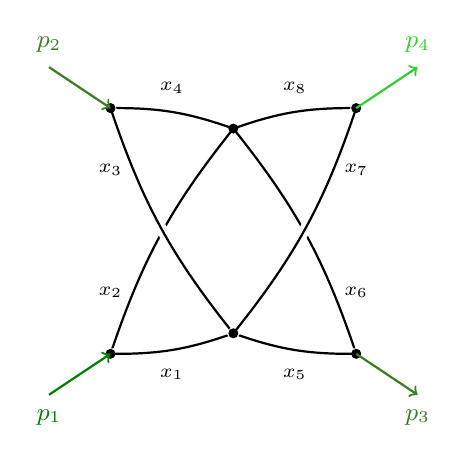
\begin{tikzpicture}[scale=.52]
 \coordinate (v1) at (2,2);
 \coordinate (v2) at (2,8);
 \coordinate (v3) at (8,2);
 \coordinate (v4) at (8,8);
 \coordinate (v5) at (5,2.5);
 \coordinate (v6) at (5,7.5);

 % Square embedding used in the original wide-angle analysis.
 \draw[hrf internal] (v6) to[bend right=10] (v1);
 \draw[hrf internal] (v6) to[bend right=10] (v2);
 \draw[hrf internal] (v6) to[bend left=10] (v3);
 \draw[hrf internal] (v6) to[bend left=10] (v4);
 % White underlays distinguish crossings from vertices.
 \foreach \a/\b/\bend in {v5/v1/left,v5/v2/left,v5/v3/right,v5/v4/right}{
   \draw[white,line width=4pt] (\a) to[bend \bend=10] (\b);
   \draw[hrf internal] (\a) to[bend \bend=10] (\b);
 }

 \node[hrf edge label] at (3.5,1.5) {$x_1$};
 \node[hrf edge label] at (2,3.5) {$x_2$};
 \node[hrf edge label] at (2,6.5) {$x_3$};
 \node[hrf edge label] at (3.5,8.5) {$x_4$};
 \node[hrf edge label] at (6.5,1.5) {$x_5$};
 \node[hrf edge label] at (8,3.5) {$x_6$};
 \node[hrf edge label] at (8,6.5) {$x_7$};
 \node[hrf edge label] at (6.5,8.5) {$x_8$};

 \foreach \v in {1,...,6} \node[hrf vertex] at (v\v) {};
 \draw[->,thick,Green] (.5,1)--(v1);
 \draw[->,thick,OliveGreen] (.5,9)--(v2);
 \draw[->,thick,OliveGreen] (v3)--(9.5,1);
 \draw[->,thick,LimeGreen] (v4)--(9.5,9);
 \node[hrf leg label,text=Green] at (.5,.45) {$p_1$};
 \node[hrf leg label,text=OliveGreen] at (.5,9.55) {$p_2$};
 \node[hrf leg label,text=OliveGreen] at (9.5,.45) {$p_3$};
 \node[hrf leg label,text=LimeGreen] at (9.5,9.55) {$p_4$};
\end{tikzpicture}
\caption{The three-loop Crown with the Schwinger-parameter assignment used in
Eq.~\eqref{eq:crown-edges}.  The external-arrow colours are visual label
guides only.}
\label{fig:crown-graph}
\end{figure}

At fixed parameters the leading polynomial is
\begin{align}
 \mathcal F_0={}&
 \SLcolour{s_{12}(x_4x_5-x_3x_6)(x_2x_7-x_1x_8)}
 \nonumber\\
 &\hspace{22mm}
 \SLcolour{-s_{23}(x_2x_3-x_1x_4)(x_6x_7-x_5x_8)}.
 \label{eq:crown-F0}
\end{align}
Regard the graph as four two-edge paths between vertices 5 and 6.  Factoring
one positive Schwinger scale from each path leaves the four ratios
\begin{equation}
 r_A=\frac{x_1}{x_2},\qquad r_B=\frac{x_3}{x_4},\qquad
 r_C=\frac{x_5}{x_6},\qquad r_D=\frac{x_7}{x_8}.
 \label{eq:crown-path-ratios}
\end{equation}
Then
\begin{align}
 \mathcal F_0&=x_2x_4x_6x_8\,\Psi_C(\boldsymbol r),\nonumber\\
 \Psi_C(\boldsymbol r)
 &=s_{12}(r_C-r_B)(r_D-r_A)
   -s_{23}(r_B-r_A)(r_D-r_C)
   =\frac12\boldsymbol r^T K_C\boldsymbol r,
 \label{eq:crown-ratio-quadratic}\\[-1mm]
 K_C&=\begin{pmatrix}
 0&s_{12}&-s_{12}-s_{23}&s_{23}\\
 s_{12}&0&s_{23}&-s_{12}-s_{23}\\
 -s_{12}-s_{23}&s_{23}&0&s_{12}\\
 s_{23}&-s_{12}-s_{23}&s_{12}&0
 \end{pmatrix}.
 \nonumber
\end{align}
The ratio Landau equations are \(K_C\boldsymbol r=0\).  Every row of \(K_C\)
sums to zero, while in the domain~\eqref{eq:crown-domain} a principal
three-by-three minor is nonzero:
\begin{equation}
 \det (K_C)_{1\ldots3,1\ldots3}
 =-2s_{12}s_{23}(s_{12}+s_{23})\ne0.
 \label{eq:crown-ratio-rank}
\end{equation}
Consequently \(K_C\) has rank three and its complete stationary locus is
\begin{equation}
 \boldsymbol r=\rho(1,1,1,1),\qquad \rho>0,
 \qquad \Psi_C(\boldsymbol r)=0.
 \label{eq:crown-ratio-stationarity}
\end{equation}
The last equality follows directly from
\(\Psi_C=\boldsymbol r^TK_C\boldsymbol r/2\).  Thus a positive stationary
family exists at every generic point of the physical wide-angle domain; no
additional kinematic condition is required.  This ratio change is the
rescaling step that precedes a local dissection of the Crown pinch.  It turns
each binomial factor in~\eqref{eq:crown-F0} into a positive path scale times
a linear difference of two ratio points.  Their common zero is
\(r_A=r_B=r_C=r_D\), which is fixed by only three relative distances, for
example \(r_B-r_A\), \(r_C-r_A\) and \(r_D-r_A\).  The four displayed
binomial constraints therefore contain only three independent equations.
Hence
\begin{equation}
 \mathcal F_\star=\mathcal F_0=\FSL,
 \qquad \FObs=0.
 \label{eq:crown-no-obstruction}
\end{equation}
Writing \(\mathcal F=\mathcal F_0+\delta\mathcal F_1+\cdots\), the certified
vector and weights are
\begin{equation}
 \vHR=(-1,-1,-1,-1,-1,-1,-1,-1;1),
 \qquad (\WSL,\WHR)=(-4,-3).
 \label{eq:crown-vector}
\end{equation}
Consequently
\begin{equation}
 \mathcal P(\delta^{-1}\x,\delta)
 =\delta^{-4}\SLcolour{\mathcal F_0}
 +\delta^{-3}\HRcolour{\bigl(\mathcal F_1+\mathcal U\bigr)}
 +\Othercolour{\mathcal O(\delta^{-2})}.
 \label{eq:crown-colours}
\end{equation}
The algorithmic lesson is the most elementary one: HRF must keep a
simultaneous positive zero of several cancellation factors.  No obstruction,
non-uniform scaling or preliminary alignment is needed.

\subsubsection{Boundary descendants: SuperCrown and HyperCrown}
\label{sec:example-crown-boundaries}

Higher-loop graphs inherit the seed on contraction strata.  In edge
order, the two graphs are
\begin{align}
E_{SC}={}&\{(1,5),(1,6),(2,7),(2,6),(3,5),(3,8),
 (4,7),(4,8),(5,7),(6,8),(7,8),(5,6)\},
\nonumber\\
E_{HC}={}&\{(1,5),(1,6),(4,9),(4,6),(2,7),(2,6),
 (3,8),(3,6),(9,5),(7,8),(8,9),(5,7)\}.
\label{eq:crown-descendant-edges}
\end{align}
In this subsection the displayed graphs use the one-based order
\(x_1,\ldots,x_{12}\).  The accompanying notebooks use
\(x_0,\ldots,x_{11}\), so that
\(x_j^{\rm notebook}=x_{j+1}^{\rm here}\).  We give both conventions when
specifying a boundary; this prevents a contraction label from being confused
with a scaling component.

\begin{figure}[htbp]
\centering
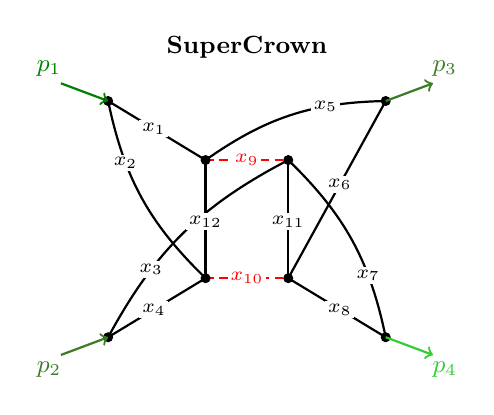
\begin{tikzpicture}[scale=.75]
 \coordinate (v1) at (-2.35,2.00);
 \coordinate (v2) at (-2.35,-2.00);
 \coordinate (v3) at (2.35,2.00);
 \coordinate (v4) at (2.35,-2.00);
 \coordinate (v5) at (-0.70,1.00);
 \coordinate (v6) at (-0.70,-1.00);
 \coordinate (v7) at (0.70,1.00);
 \coordinate (v8) at (0.70,-1.00);
 \node[font=\small\bfseries] at (0,2.90) {SuperCrown};

 \draw[hrf internal] (v1)--node[hrf edge label,pos=.47] {$x_1$}(v5);
 \draw[hrf internal] (v1) to[bend right=17]
   node[hrf edge label,pos=.30] {$x_2$}(v6);
 \draw[hrf internal] (v2) to[bend left=17]
   node[hrf edge label,pos=.30] {$x_3$}(v7);
 \draw[hrf internal] (v2)--node[hrf edge label,pos=.47] {$x_4$}(v6);
 \draw[hrf internal] (v3) to[bend right=17]
   node[hrf edge label,pos=.30] {$x_5$}(v5);
 \draw[hrf internal] (v3)--node[hrf edge label,pos=.47] {$x_6$}(v8);
 \draw[hrf internal] (v4) to[bend right=17]
   node[hrf edge label,pos=.30] {$x_7$}(v7);
 \draw[hrf internal] (v4)--node[hrf edge label,pos=.47] {$x_8$}(v8);
 \draw[hrf contracted] (v5)--node[hrf edge label,pos=.50,text=red] {$x_9$}(v7);
 \draw[hrf contracted] (v6)--node[hrf edge label,pos=.50,text=red] {$x_{10}$}(v8);
 \draw[hrf internal] (v7)--node[hrf edge label,pos=.52] {$x_{11}$}(v8);
 \draw[hrf internal] (v5)--node[hrf edge label,pos=.52] {$x_{12}$}(v6);

 \foreach \v in {1,...,8} \node[hrf vertex] at (v\v) {};
 \draw[->,thick,Green] (-3.15,2.30)--(v1);
 \draw[->,thick,OliveGreen] (-3.15,-2.30)--(v2);
 \draw[->,thick,OliveGreen] (v3)--(3.15,2.30);
 \draw[->,thick,LimeGreen] (v4)--(3.15,-2.30);
 \node[hrf leg label,text=Green] at (-3.35,2.55) {$p_1$};
 \node[hrf leg label,text=OliveGreen] at (-3.35,-2.55) {$p_2$};
 \node[hrf leg label,text=OliveGreen] at (3.35,2.55) {$p_3$};
 \node[hrf leg label,text=LimeGreen] at (3.35,-2.55) {$p_4$};
\end{tikzpicture}
\hspace{10mm}
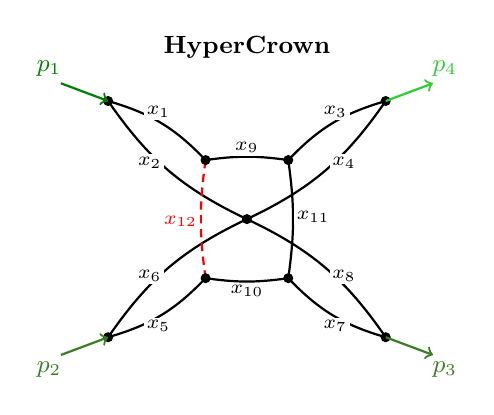
\begin{tikzpicture}[scale=.75]
 \coordinate (v1) at (-2.35,2.00);
 \coordinate (v2) at (-2.35,-2.00);
 \coordinate (v4) at (2.35,2.00);
 \coordinate (v3) at (2.35,-2.00);
 \coordinate (v5) at (-0.70,1.00);
 \coordinate (v9) at (0.70,1.00);
 \coordinate (v8) at (0.70,-1.00);
 \coordinate (v7) at (-0.70,-1.00);
 \coordinate (v6) at (0,0);

 \node[font=\small\bfseries] at (0,2.90) {HyperCrown};

 % Upper-left pair
 \draw[hrf internal]
   (v1) to[bend left=15]
   node[hrf edge label,pos=.47,above] {$x_1$} (v5);
 \draw[hrf internal]
   (v1) to[bend right=15]
   node[hrf edge label,pos=.35,below] {$x_2$} (v6);

 % Upper-right pair
 \draw[hrf internal]
   (v4) to[bend right=15]
   node[hrf edge label,pos=.47,above] {$x_3$} (v9);
 \draw[hrf internal]
   (v4) to[bend left=15]
   node[hrf edge label,pos=.35,below] {$x_4$} (v6);

 % Lower-left pair
 \draw[hrf internal]
   (v2) to[bend right=15]
   node[hrf edge label,pos=.47,below] {$x_5$} (v7);
 \draw[hrf internal]
   (v2) to[bend left=15]
   node[hrf edge label,pos=.35,above] {$x_6$} (v6);

 % Lower-right pair
 \draw[hrf internal]
   (v3) to[bend left=15]
   node[hrf edge label,pos=.47,below] {$x_7$} (v8);
 \draw[hrf internal]
   (v3) to[bend right=15]
   node[hrf edge label,pos=.35,above] {$x_8$} (v6);

 % Inner quadrilateral: gently curved outwards
 \draw[hrf internal]
   (v9) to[bend right=8]
   node[hrf edge label,pos=.50,above] {$x_9$} (v5);
 \draw[hrf internal]
   (v7) to[bend right=8]
   node[hrf edge label,pos=.50,below] {$x_{10}$} (v8);
 \draw[hrf internal]
   (v8) to[bend right=8]
   node[hrf edge label,pos=.52,right] {$x_{11}$} (v9);
 \draw[hrf contracted]
   (v5) to[bend right=8]
   node[hrf edge label,pos=.52,left,text=red] {$x_{12}$} (v7);

 \foreach \v in {1,...,9}
   \node[hrf vertex] at (v\v) {};

 % External legs
 \draw[->,thick,Green]
   (-3.15,2.30)--(v1);
 \draw[->,thick,OliveGreen]
   (-3.15,-2.30)--(v2);
 \draw[->,thick,OliveGreen]
   (v3)--(3.15,-2.30);
 \draw[->,thick,LimeGreen]
   (v4)--(3.15,2.30);

 \node[hrf leg label,text=Green]
   at (-3.35,2.55) {$p_1$};
 \node[hrf leg label,text=OliveGreen]
   at (-3.35,-2.55) {$p_2$};
 \node[hrf leg label,text=OliveGreen]
   at (3.35,-2.55) {$p_3$};
 \node[hrf leg label,text=LimeGreen]
   at (3.35,2.55) {$p_4$};
\end{tikzpicture}
\caption{Higher-loop Crown descendants: the five-loop SuperCrown (left) and
the four-loop HyperCrown (right).  Red dashed edges are set to zero on the
representative contraction strata used below: \(x_9=x_{10}=0\) for the
SuperCrown and \(x_{12}=0\) for the HyperCrown, in the one-based convention
of the figure.}
\label{fig:crown-descendant-graphs}
\end{figure}

\paragraph{SuperCrown: a codimension-two inherited Crown.}

The focused boundary is
\begin{equation}
 B_{\rm SC}=\{x_9=x_{10}=0\}_{\rm here}
 =\{x_8=x_9=0\}_{\rm notebook}.
 \label{eq:SC-boundary}
\end{equation}
After restriction, the surviving superleading polynomial is not merely the
Crown polynomial: it includes the two additional active edge parameters,
\begin{equation}
 \mathcal F_{\rm SL}^{\rm SC}
 =x_{11}x_{12}\,\mathcal F_{\rm SL}^{C}(x_1,\ldots,x_8),
 \qquad \mathcal F_{\rm Obs}^{\rm SC}=0.
 \label{eq:SC-decomposition}
\end{equation}
Equivalently, its two generators are
\begin{align}
 g_1&=(x_4x_5-x_3x_6)(x_2x_7-x_1x_8),\\
 g_2&=(x_2x_3-x_1x_4)(x_6x_7-x_5x_8),
 \label{eq:SC-generators}
\end{align}
with the same simultaneous positive component as the Crown.  In the active
order \((x_1,\ldots,x_8,x_{11},x_{12})\), the certified augmented vector is
\begin{equation}
 \vHR^{\rm SC}=(-1,-1,-1,-1,-1,-1,-1,-1,-1,-1;1),
 \qquad (\WSL,\WHR)=(-6,-5).
 \label{eq:SC-vector}
\end{equation}
The weights include the monomial factor \(x_{11}x_{12}\); stripping it would
incorrectly quote the Crown weights \((-4,-3)\).  The current polynomial-factor
run finds one HR on this stratum with no search truncation.

\paragraph{HyperCrown: two boundary-HR types.}

For the HyperCrown the four edges
\begin{equation}
 Q_{\rm HC}=\{x_9,x_{10},x_{11},x_{12}\}_{\rm here}
 =\{x_8,x_9,x_{10},x_{11}\}_{\rm notebook}
\end{equation}
form a square with dihedral symmetry \(D_4\).  External, edge and kinematic
labels are permuted together.  Consequently one direct positive witness
establishes its entire orbit, including crossing-related representatives.
The wide-angle results through codimension two are
\begin{center}
\small
\begin{tabular}{@{}
 >{\raggedright\arraybackslash}p{0.10\textwidth}
 >{\raggedright\arraybackslash}p{0.18\textwidth}
 >{\raggedright\arraybackslash}p{0.30\textwidth}
 >{\raggedright\arraybackslash}p{0.33\textwidth}@{}}
\toprule
Type & Representative boundary & Certified scaling & Full orbit / conclusion\\
\midrule
I & \(x_{12}=0\) & the opposite edge \(x_{11}\) has \(v_{11}=-2\);
all other active \(v_e=-1\); \((\WSL,\WHR)=(-6,-5)\)
& \(x_9=0\), \(x_{10}=0\), \(x_{11}=0\), \(x_{12}=0\): one HR on each boundary\\[1mm]
II & \(x_9=x_{11}=0\) & all ten active components have \(v_e=-1\);
\((\WSL,\WHR)=(-5,-4)\)
& \(\{x_9,x_{11}\}\), \(\{x_{10},x_{11}\}\),
\(\{x_{10},x_{12}\}\), \(\{x_9,x_{12}\}\): one HR on each boundary\\[1mm]
Excluded & \(x_9=x_{10}=0\) & no exact coverage vector & the opposite-pair
orbit \(\{x_9,x_{10}\}\), \(\{x_{11},x_{12}\}\) has no HR\\
\bottomrule
\end{tabular}
\end{center}
Here every boundary equation means \(x_e=0\); it must not be read as a value
of \(v_e\).  Type~I has the decomposition
\begin{equation}
 \left.\mathcal F_0^{\rm HC}\right|_{x_{12}=0}
 =\underbrace{\left[\mathcal F_0^{\rm HC}\right]_{W=-6}}_{\mathcal F_{\rm SL}^{\rm I}
 =x_{11}Q_{\rm I}}
 +\underbrace{\left[\mathcal F_0^{\rm HC}\right]_{W=-5}}_{\mathcal F_{\rm Obs}^{\rm I}},
 \label{eq:HC-type-I-decomposition}
\end{equation}
where the bracket selects monomials by the displayed Type-I vector.  The
positive zero of \(Q_{\rm I}\), together with its derivative conditions, is
the Landshoff cancellation locus; the obstruction fixes the extra unit of
scaling on the opposite square edge.  For Type~II every surviving term of
\(\mathcal F_0^{\rm HC}\) has weight \(-5\), so
\begin{equation}
 \left.\mathcal F_0^{\rm HC}\right|_{x_9=x_{11}=0}
 =\mathcal F_{\rm SL}^{\rm II},
 \qquad \mathcal F_{\rm Obs}^{\rm II}=0.
 \label{eq:HC-type-II-decomposition}
\end{equation}
The two accepted generator presentations recorded for a direct Type-II
representative give the same positive component and the same vector; they are
one physical HR, not two.
The momentum reconstruction gives the complementary interpretation.  Type~I
is the four-jet Landshoff flow with one additional soft loop carried by the
opposite square edge.  Type~II instead adds one loop collinear to an external
direction.  Neither type requires a generic-angle Glauber mode.

The opposite-pair exclusion is stronger than a failed capped search.  On
the notebook boundary \(x_8=x_9=0\), complete factorisation of all relevant
derivatives and primitive kinematic-channel polynomials produces one
\(s_{12}\)-supported Crown-like generator and no \(s_{23}\)-supported
companion.  Exact coverage rejects the remaining one-generator presentation,
with no candidate, union, polynomial-size or solver cap.  Its \(D_4\) image
excludes \(x_{10}=x_{11}=0\).  By contrast, the HyperCrown interior is still
unresolved: the completed capped trials contain no HR, but the cap and a
timeout prohibit an absence claim.

The family therefore adds two indispensable capabilities.  First, the
search must descend to contraction strata: an interior-only analysis misses
regions present in the parent integral.  Second, constructive witnesses and
negative statements require different standards.  Symmetry can complete an
existence orbit, whereas absence requires a complete polynomial-factor and
exact-scaling audit with every search budget exposed.

\subsubsection{The four-loop No-Crown converse}

The converse wide-angle audit completes the four-loop picture.  Sixteen
mixed-sign topologies without a Crown contraction minor have no interior or
boundary HR.  The search is complete on the stated graph sample, so these are
no-HR certificates rather than failures to find a candidate.  Together with
the positive Crown descendants above, this establishes both directions of
the Crown-minor criterion for the audited wide-angle topologies through four
loops.

\subsubsection{The Crown family in Regge limits: an audited correspondence}
\label{sec:crown-wide-angle-regge}

The Regge comparison becomes meaningful only after both sides of the
wide-angle classification are visible.  Momentum conservation gives
\(s_{13}=-s_{12}-s_{23}\), and the three channel charts used in the audit are
\begin{align}
 T_{23}:&\quad s_{23}=-\delta s_{12}, &&s_{12}>0,\nonumber\\
 T_{12}:&\quad s_{12}=-\delta s_{23}, &&s_{23}<0,\nonumber\\
 T_{13}:&\quad s_{23}=-s_{12}+\delta s_{12}, &&s_{12}>0,
 \label{eq:crown-regge-charts}
\end{align}
with \(\delta\to0^+\).  In the ratio coordinates of
Eq.~\eqref{eq:crown-path-ratios}, the leading Crown polynomial in each chart
is, up to a nonzero kinematic and positive monomial factor,
\begin{align}
 \Psi_C^{T_{23}}&\propto(r_C-r_B)(r_D-r_A),\nonumber\\
 \Psi_C^{T_{12}}&\propto(r_B-r_A)(r_D-r_C),\nonumber\\
 \Psi_C^{T_{13}}&\propto(r_C-r_A)(r_D-r_B).
 \label{eq:crown-regge-ratio-factors}
\end{align}
The corresponding positive cancellation loci are therefore
\begin{align}
 T_{23}:&\quad r_B=r_C,\quad r_A=r_D,\nonumber\\
 T_{12}:&\quad r_A=r_B,\quad r_C=r_D,\nonumber\\
 T_{13}:&\quad r_A=r_C,\quad r_B=r_D.
 \label{eq:crown-regge-loci}
\end{align}
This exposes an important change in codimension.  At generic wide angle the
Crown locus identifies all four ratio points and hence has three independent
relative-distance equations.  In each Regge chart the leading polynomial
reduces to one product of two difference factors, leaving only two independent
equations.  Each Regge locus is therefore larger and contains the wide-angle diagonal
\(r_A=r_B=r_C=r_D\).

Nevertheless, the reduction from three equations to two does not produce
new seed topologies in the completed low-loop survey.  The positive side is
inherited by every audited graph that exposes a Crown contraction minor: the
Crown itself has an HR in all three channels, and its higher-loop descendants
carry the corresponding region on the contraction stratum.  On the negative
side, the same sixteen four-loop No-Crown topologies were checked in
\(T_{23}\), \(T_{12}\) and \(T_{13}\).  All 48 interiors and all 343356
nonempty contraction strata through \(E-2\) were resolved, with no HR.

Thus, after the channel relabellings implied by crossing, the set of
topologies with a Regge HR agrees exactly with the set having a wide-angle
Landshoff HR at three and four loops.  Equivalently, in this complete audited
sample both are precisely the topologies containing the Crown as a
contraction minor.  We call this the wide-angle-to-Regge conjecture when
extrapolated beyond four loops.  Its validity is not a trivial consequence
of the Landau equations: algebraically the Regge pinch requires fewer
conditions and could have admitted additional topologies, but none occurs in
the completed survey.

\subsection{Five-point integrals: the fish seed}
\label{sec:example-five-point}

The examples below use the same unlabeled two-loop six-propagator
topology but different external attachments and different kinematic
expansions.  We refer to this topology as the fish seed.  The first is the
spacelike-collinear limit for which this seed
was originally identified.  The second is an exactly on-shell approach to
the planar boundary of five-particle wide-angle scattering.  The
cancellation ideals and total vectors are different, but in both cases the
same sparse topology supports an HR.  A central-soft multi-Regge limit
reaches the normalized planar boundary by a different route and supplies a
third certificate.  The three cancellation mechanisms should not be
identified merely because the unlabeled graph is common.  Before applying
the seed to near-planar scattering, we define the underlying massless
five-point kinematics separately, since that construction is independent of
the graph and its loop order.

\subsubsection{The spacelike-collinear limit}
\label{sec:five-point-spacelike-collinear}

The spacelike-collinear application of HRF was presented in the recent short
publication~\cite{Chen:2026dnj}.  We use there, and here, the kinematic
parametrisation introduced in Ref.~\cite{Henn:2024qjq}, which originates from
a momentum-twistor construction.  It makes the dependence on the transverse
collinear variable \(\delta\) especially transparent: the deformation away
from the strict collinear surface enters linearly through \(c\delta\), while
the vanishing collinear invariant starts at \(s_{23}=-4\delta^2\).  Thus the
Mandelstam invariants are polynomial, and at most quadratic, in the expansion
variable.  In our notation the collinear chart is
\begin{equation}
 \begin{gathered}
 s_{12}=sz,\qquad s_{23}=-4\delta^2,\qquad
 s_{34}=-s\chi(z-1),\\
 s_{45}=s,\qquad s_{15}=s\chi+c\delta,\qquad \delta\to0^+,
 \end{gathered}
 \label{eq:five-kinematics}
\end{equation}
with
\begin{equation}
 s>0,\qquad z>1,\qquad -1<\chi<0,
 \label{eq:five-domain}
\end{equation}
and fixed nonzero \(c\).  Keeping \(\chi\) negative is useful: the same
variables then display directly the change from timelike to spacelike
collinear kinematics.

The two-loop seed has edge set
\begin{equation}
 E_5=\{(1,3),(1,5),(2,3),(2,5),(3,4),(4,5)\}
 \longleftrightarrow (x_1,\ldots,x_6),
 \label{eq:five-edges}
\end{equation}
and external attachment \(p_i\to i\), \(i=1,\ldots,5\).  We use
\(x_{i,j,\ldots}=x_ix_j\cdots\).

\begin{figure}[htbp]
\centering
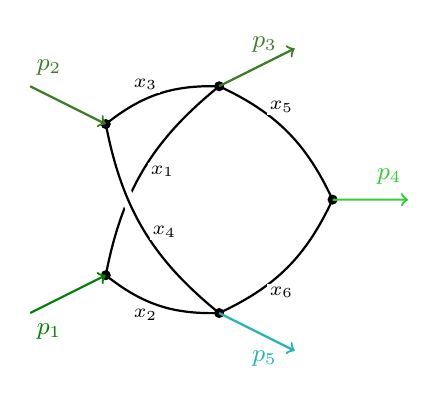
\begin{tikzpicture}[scale=.48]
 \coordinate (v1) at (2,3);
 \coordinate (v2) at (2,7);
 \coordinate (v3) at (5,8);
 \coordinate (v4) at (8,5);
 \coordinate (v5) at (5,2);

 \draw[hrf internal] (v3) to[bend right=20] (v1);
 \draw[hrf internal] (v3) to[bend right=20] (v2);
 \draw[white,double=white,double distance=3pt,thick]
   (v5) to[bend left=20] (v2);
 \draw[hrf internal] (v5) to[bend left=20] (v2);
 \draw[hrf internal] (v5) to[bend left=20] (v1);
 \draw[hrf internal] (v3) to[bend left=20] (v4);
 \draw[hrf internal] (v5) to[bend right=20] (v4);

 \foreach \v in {1,...,5} \node[hrf vertex] at (v\v) {};
 \draw[->,thick,Green] (0,2)--(v1);
 \draw[->,thick,OliveGreen] (0,8)--(v2);
 \draw[->,thick,OliveGreen] (v3)--(7,9);
 \draw[->,thick,LimeGreen] (v4)--(10,5);
 \draw[->,thick,TealBlue] (v5)--(7,1);

 \node[hrf leg label,text=Green] at (.5,1.5) {$p_1$};
 \node[hrf leg label,text=OliveGreen] at (.5,8.5) {$p_2$};
 \node[hrf leg label,text=OliveGreen] at (6.2,9.1) {$p_3$};
 \node[hrf leg label,text=LimeGreen] at (9.5,5.6) {$p_4$};
 \node[hrf leg label,text=TealBlue] at (6.2,.8) {$p_5$};

 \node[hrf edge label] at (3.50,5.75) {$x_1$};
 \node[hrf edge label] at (3.05,1.95) {$x_2$};
 \node[hrf edge label] at (3.05,8.05) {$x_3$};
 \node[hrf edge label] at (3.55,4.15) {$x_4$};
 \node[hrf edge label] at (6.65,7.45) {$x_5$};
 \node[hrf edge label] at (6.65,2.55) {$x_6$};
\end{tikzpicture}
\caption{The two-loop five-point seed graph, redrawn in the style of
Ref.~\cite{Chen:2026dnj}, with the Schwinger parameters used in
Eqs.~\eqref{eq:five-facet-F0}--\eqref{eq:five-HR-Fdelta}.}
\label{fig:five-point-seed}
\end{figure}

\paragraph{The ordinary facet and the hidden region.}

For the ordinary facet vector
\begin{equation}
 \vec v_C=(-2,0,-2,-2,-2,0;1),
 \label{eq:five-facet-vector}
\end{equation}
the expanded polynomial is classified as
\begin{align}
 \mathcal F_0^{[C]}={}&
 \HRcolour{s\bigl(x_{2,5}+\chi x_{1,6}\bigr)
       \bigl[(z-1)x_3-x_4\bigr]}
 +\Othercolour{sz(\chi+1)x_{2,3,6}},
 \label{eq:five-facet-F0}\\
 \mathcal F_\delta^{[C]}={}&
 \Othercolour{-c\delta x_{1,4,6}+c\delta x_{2,3,6}}
 +\HRcolour{4\delta^2x_{1,4,5}}
 \Othercolour{-4\delta^2x_{2,3,5}}.
 \label{eq:five-facet-Fdelta}
\end{align}
There is no red sector: the blue monomials form an ordinary lower facet.

For the hidden-region vector
\begin{equation}
 \vHR=(-2,-1,-2,-2,-2,-1;1),
 \qquad (\WSL,\WHR)=(-5,-4),
 \label{eq:five-HR-vector}
\end{equation}
the identical polynomial instead reads
\begin{align}
 \mathcal F_0^{[\HR]}={}&
 \underbrace{\SLcolour{s\bigl(x_{2,5}+\chi x_{1,6}\bigr)
       \bigl[(z-1)x_3-x_4\bigr]}}_{\FSL}
 +\underbrace{\HRcolour{sz(\chi+1)x_{2,3,6}}}_{\FObs},
 \label{eq:five-HR-F0}\\
 \mathcal F_\delta^{[\HR]}={}&
 \HRcolour{-c\delta x_{1,4,6}}
 +\Othercolour{c\delta x_{2,3,6}}
 +\HRcolour{4\delta^2x_{1,4,5}}
 \Othercolour{-4\delta^2x_{2,3,5}}.
 \label{eq:five-HR-Fdelta}
\end{align}
The cancellation ideal is generated by
\begin{equation}
 f_1=x_{2,5}+\chi x_{1,6},\qquad
 f_2=(z-1)x_3-x_4,\qquad \ideal=\langle f_1,f_2\rangle.
 \label{eq:five-generator}
\end{equation}
The red product vanishes at the positive pinch.  The blue obstruction,
the blue kinematically suppressed terms, and
\begin{equation}
 \mathcal U_{\WHR}
 =\HRcolour{x_{1,3}+x_{1,4}+x_{1,5}+x_{3,5}+x_{4,5}}
 \label{eq:five-U-leading}
\end{equation}
form the physical layer.  This example introduces the obstruction:
\(\FObs\ne0\) fixes a non-uniform scaling that would not be determined by
the factorized cancellation sector alone.

\paragraph{Complete momentum flow.}

Table~\ref{tab:five-sc-edge-flow} gives the edge assignment for both the
ordinary facet and the HR.  The momentum \(q_e\) flows through the edge
carrying \(x_e\), and each triple denotes the exponents of
\((q_e^+,q_e^-,|q_{e\perp}|)\).  The last column in each case is the power
\(\kappa_e\) of \(q_e^2\).
\begin{table}[htbp]
\centering
\small
\begin{tabular}{@{}c cc cc@{}}
\toprule
& \multicolumn{2}{c}{facet \(\vec v_C\)}
& \multicolumn{2}{c}{hidden \(\vHR\)}\\
\cmidrule(lr){2-3}\cmidrule(l){4-5}
edge & \((a_e,b_e,c_e)\) & \(\kappa_e\)
     & \((a_e,b_e,c_e)\) & \(\kappa_e\)\\
\midrule
\(q_1\) & \((0,2,1)\) & 2 & \((1,1,1)\) & 2\\
\(q_2\) & \((0,0,1)\) & 0 & \((1,0,1)\) & 1\\
\(q_3\) & \((0,2,1)\) & 2 & \((0,2,1)\) & 2\\
\(q_4\) & \((0,2,1)\) & 2 & \((0,2,1)\) & 2\\
\(q_5\) & \((0,2,1)\) & 2 & \((1,1,1)\) & 2\\
\(q_6\) & \((0,0,0)\) & 0 & \((0,0,0)\) & 1\\
\bottomrule
\end{tabular}
\caption{Complete edge-momentum valuations for the five-point
spacelike-collinear facet and HR.  Edge \(q_e\) corresponds to parameter
\(x_e\) in Fig.~\ref{fig:five-point-seed}.}
\label{tab:five-sc-edge-flow}
\end{table}

In the facet region the table admits a homogeneous collinear loop basis and
no transverse-dominated loop rerouting.  In the HR, \(q_1\) and \(q_5\) are
separately soft.  Vertex conservation forces the minus components to cancel
in the independent rerouting
\begin{equation}
 \ell_G=q_1-q_5\sim(\delta,\delta^2,\delta),
 \label{eq:five-sc-glauber-rerouting}
\end{equation}
while one may take \(\ell_s=q_1\sim(\delta,\delta,\delta)\) as the other
loop variable.  Thus the HR has one soft and one Glauber loop.  The entry for
\(q_6\) is cancellation enhanced: its leading longitudinal and transverse
terms cancel so that \(q_6^2\sim\delta\), despite all three components being
of order one.  This coefficient-level structure is known explicitly in the
spacelike-collinear solution, so this reconstruction is mode complete.

\paragraph{Parameter- and momentum-space power counting.}

For unit propagator powers, the scalar LP representation contains
\(\mathcal P^{-D/2}\).  The edge-vector sum is
\(\sum_e v_e=-10\).  Only a restricted neighbourhood of the cancellation
locus contributes: in local coordinates one cancellation-normal variable
has one power less support than a generic variable with the same edge
scaling.  The parameter measure is therefore
\begin{equation}
 \delta^{-10}\,\delta^{+1}=\delta^{-9}.
 \label{eq:five-sc-parameter-measure}
\end{equation}
Since the resolved LP polynomial has weight \(-4\),
\(\mathcal P^{-D/2}\sim\delta^{2D}\), and hence
\begin{equation}
 I_{\rm SC}^{\rm scalar}\sim
 \delta^{-9+2D}=\delta^{-1-4\epsilon},
 \qquad D=4-2\epsilon.
 \label{eq:five-sc-parameter-power}
\end{equation}
The power enhancement is a property of the unit-numerator scalar integral.
For the gauge-theory numerator relevant to the amplitude, one additional
power of \(\delta\) gives the leading-power behaviour
\(\delta^{-4\epsilon}\).

The same count is obtained in momentum space.  A convenient routing contains
one soft loop and one Glauber loop,
\begin{equation}
 \ell_s\sim(\delta,\delta,\delta),
 \qquad
 \ell_G\sim(\delta,\delta^2,\delta),
 \label{eq:five-sc-modes}
\end{equation}
where the entries denote \((q^+,q^-,|q_\perp|)\).  Their measures scale as
\(\delta^D\) and \(\delta^{D+1}\), respectively.  The six propagator
virtualities have powers
\begin{equation}
 (2,1,2,2,2,1),
 \label{eq:five-sc-virtualities}
\end{equation}
whose sum is ten.  Therefore
\begin{equation}
 I_{\rm SC}^{\rm scalar}\sim
 \delta^{D+(D+1)-10}=\delta^{-1-4\epsilon},
 \label{eq:five-sc-momentum-power}
\end{equation}
in agreement with Eq.~\eqref{eq:five-sc-parameter-power}.  In the original
edge routing the Glauber momentum is the difference of two soft edge
momenta.  This is why inspection of individual propagator modes alone does
not reveal it.

\subsubsection{A vertex correction: a genuinely non-binomial generator}

The same kinematics applied to the three-loop vertex-corrected graph gives
\begin{equation}
 \begin{split}
 E_{5V}={}&\{(1,3),(1,5),(3,7),(6,5),(3,4),\\[-1mm]
          &\hspace{17mm}(4,5),(2,7),(6,7),(2,6)\}
 \longleftrightarrow (x_0,\ldots,x_8).
 \end{split}
 \label{eq:five-vertex-edges}
\end{equation}

\begin{figure}[htbp]
\centering
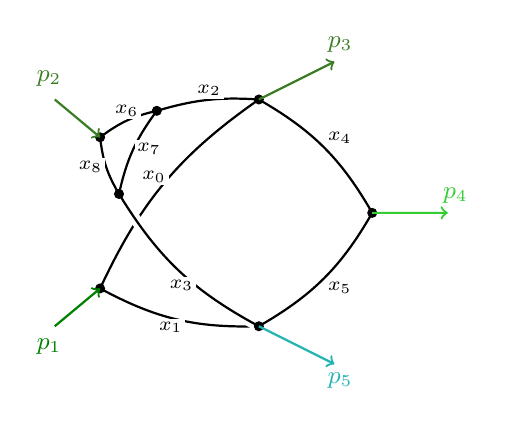
\begin{tikzpicture}[scale=.48]

 \coordinate (v1) at (0.8,3);
 \coordinate (v2) at (0.8,7);
 \coordinate (v3) at (5,8);
 \coordinate (v4) at (8,5);
 \coordinate (v5) at (5,2);
 \coordinate (v7) at (2.3,7.7);
 \coordinate (v6) at (1.3,5.5);

 % Main graph: the bends point away from its centre.
 \draw[hrf internal]
   (v1) to[bend left=15]
   node[hrf edge label,pos=.53,left] {$x_0$} (v3);
 \draw[hrf internal]
   (v1) to[bend right=15]
   node[hrf edge label,pos=.46,below] {$x_1$} (v5);
 \draw[hrf internal]
   (v7) to[bend left=10]
   node[hrf edge label,pos=.52,above] {$x_2$} (v3);

 % White underlay preserves the non-vertex crossing.
 \draw[white,line width=4pt]
   (v6) to[bend right=15] (v5);
 \draw[hrf internal]
   (v6) to[bend right=15]
   node[hrf edge label,pos=.52,below=1pt] {$x_3$} (v5);

 \draw[hrf internal]
   (v3) to[bend left=15]
   node[hrf edge label,pos=.50,above right] {$x_4$} (v4);
 \draw[hrf internal]
   (v4) to[bend left=15]
   node[hrf edge label,pos=.50,below right] {$x_5$} (v5);

 % Local vertex-correction triangle.
 \draw[hrf internal]
   (v2) to[bend left=12]
   node[hrf edge label,pos=.50,above] {$x_6$} (v7);
 \draw[hrf internal]
   (v6) to[bend left=12]
   node[hrf edge label,pos=.52,right] {$x_7$} (v7);
 \draw[hrf internal]
   (v2) to[bend right=12]
   node[hrf edge label,pos=.50,left] {$x_8$} (v6);

 \foreach \v in {1,...,7} \node[hrf vertex] at (v\v) {};
 \draw[->,thick,Green] (-.40,2)--(v1);
 \draw[->,thick,OliveGreen] (-.40,8)--(v2);
 \draw[->,thick,OliveGreen] (v3)--(7,9);
 \draw[->,thick,LimeGreen] (v4)--(10,5);
 \draw[->,thick,TealBlue] (v5)--(7,1);
 \node[hrf leg label,text=Green]
  at (-.55,1.45) {$p_1$};
\node[hrf leg label,text=OliveGreen]
  at (-.55,8.55) {$p_2$};
 \node[hrf leg label,text=OliveGreen] at (7.15,9.45) {$p_3$};
 \node[hrf leg label,text=LimeGreen] at (10.20,5.45) {$p_4$};
 \node[hrf leg label,text=TealBlue] at (7.15,.55) {$p_5$};
\end{tikzpicture}
\caption{The three-loop vertex-corrected five-point graph, drawn as the
two-loop seed of Fig.~\ref{fig:five-point-seed} with a local vertex correction
adjacent to \(p_2\).  In particular, \(x_7\) lies outside the other loops.
The labels
\(x_0,\ldots,x_8\) are those used in
Eqs.~\eqref{eq:five-vertex-factors}--\eqref{eq:five-vertex-vector}.}
\label{fig:five-point-vertex}
\end{figure}



Here a pairwise monomial search is insufficient.  A convenient primitive
generator is \(g_1g_2\), where
\begin{align}
 g_1={}&(z-1)(x_2x_6+x_2x_7+x_2x_8)+zx_6x_7
 \nonumber\\[-1mm]
 &-(x_3x_6+x_3x_7+x_3x_8+x_6x_7+x_7x_8),
 \nonumber\\
 g_2={}&x_1x_4+\chi x_0x_5.
 \label{eq:five-vertex-factors}
\end{align}
The first factor has more than two monomials and cannot be represented by a
single equality of a monomial pair.  The decomposition is nevertheless as
simple at ideal level as in the seed:
\begin{align}
 \mathcal F_\star={}&
 \underbrace{\SLcolour{-s\,g_1g_2}}_{\FSL}
 +\underbrace{\HRcolour{-s(1+\chi)z\,x_1x_5
 (x_2x_6+x_2x_7+x_6x_7+x_2x_8)}}_{\FObs},
 \label{eq:five-vertex-decomposition}\\
 \vHR={}&(-2,-1,-2,-2,-2,-1,-2,-2,-2;1),
 \qquad (\WSL,\WHR)=(-7,-6).
 \label{eq:five-vertex-vector}
\end{align}
The lesson is not merely that long factors may occur.  HRF must construct
and test the ideal generated by primitive polynomial factors, allow
polynomial multipliers in \(\FSL\), and solve the positive pinch only after
the scaling law has isolated that sector.  A binomial-only or
pair-sector-only candidate list would miss this region.

\subsubsection{Massless five-point kinematics and the near-planar expansion}
\label{sec:five-point-near-planar}

Let all five external momenta be exactly massless and keep all adjacent
Mandelstam invariants at wide angle, with the physical signs
\begin{equation}
 s_{12},s_{34},s_{45}>0,\qquad s_{23},s_{15}<0.
 \label{eq:five-wide-angle-signs}
\end{equation}
Define
\begin{equation}
 \Gamma_5=\det(2p_i\!\cdot p_j)_{i,j=1}^{4}=\epsilon_5^2,
 \qquad \epsilon_5=4i\,\varepsilon(p_1,p_2,p_3,p_4).
 \label{eq:five-gram-definition}
\end{equation}
Geometrically, \(\Gamma_5\) is the signed squared four-volume of the
parallelotope spanned by \(p_1,\ldots,p_4\), up to the conventional factor
\(2^4\); equivalently it is \(2^4(4!)^2\) times the signed squared volume of
the corresponding four-simplex.  Its vanishing is therefore the condition
that the external momenta become coplanar.  For real momenta on the physical
non-coplanar sheet, \(\epsilon_5\) is purely imaginary and \(\Gamma_5<0\).

To define the approach to this boundary, use the exact five-point variables
introduced in the MRK analysis of Ref.~\cite{Abreu:2024xoh}.  In the
\((p_1,p_2)\) light-cone frame, write the complex transverse momentum as
\(\mathbf p=p^x+ip^y\) and its conjugate as
\(\bar{\mathbf p}=p^x-ip^y\), and define
\begin{equation}
 w=-\frac{\mathbf p_3}{\mathbf p_4},\qquad
 \bar w=-\frac{\bar{\mathbf p}_3}{\bar{\mathbf p}_4},\qquad
 X_{34}=\frac{p_3^+}{p_4^+},\qquad
 X_{45}=\frac{p_4^+}{p_5^+},\qquad
 Q_4^2=|\mathbf p_4|^2.
 \label{eq:five-exact-kinematic-chart}
\end{equation}
For comparing the two expansions below it is useful to replace the inverse
transverse ratios by
\begin{equation}
 \zeta=-\frac1w=\frac{\mathbf p_4}{\mathbf p_3},\qquad
 \bar\zeta=-\frac1{\bar w}
 =\frac{\bar{\mathbf p}_4}{\bar{\mathbf p}_3}.
 \label{eq:five-zeta-chart}
\end{equation}
These four dimensionless ratios and the transverse scale \(Q_4^2\) form an
exact chart, up to an irrelevant longitudinal boost.  Transverse momentum
conservation gives
\(\mathbf p_3=-w\mathbf p_4\) and
\(\mathbf p_5=-(1-w)\mathbf p_4\), together with their barred counterparts;
on-shellness then fixes the minus components from the plus components.  In
this chart the parity-odd invariant factorises exactly as
\begin{equation}
 \epsilon_5=s_{12}Q_4^2(w-\bar w)
 =s_{12}Q_4^2\frac{\zeta-\bar\zeta}{\zeta\bar\zeta}.
 \label{eq:five-exact-parity-odd-chart}
\end{equation}
Equations~\eqref{eq:five-exact-kinematic-chart} and
\eqref{eq:five-zeta-chart} describe generic five-point kinematics before
either expansion is taken.  We shall select two distinct paths from this
same generic domain.  The near-planar path makes the angular factor
\(\zeta-\bar\zeta\) vanish at fixed \(Q_4^2\).  The central-soft MRK path
defined later instead makes \(Q_4^2\) vanish while the ratio
\(\zeta/\bar\zeta\) remains generic.  The latter is therefore not obtained
by first imposing coplanarity and then taking a soft MRK sublimit.
In the physical non-coplanar region \(\bar w=w^*\).  The near-planar
wide-angle expansion is defined by
\begin{align}
 w&=-\frac1\xi+\frac{i}{2}\lambda,&
 \bar w&=-\frac1\xi-\frac{i}{2}\lambda,\nonumber\\
 \zeta&=\frac{\xi}{1-i\xi\lambda/2},&
 \bar\zeta&=\frac{\xi}{1+i\xi\lambda/2},\nonumber\\
 &\lambda\to0^+,&
 &\xi,\ X_{34},\ X_{45},\ Q_4^2\ \text{fixed},
 \label{eq:five-near-planar-chart}
\end{align}
where \(\xi>0\).  Thus the coplanar boundary is simply
\(\zeta=\bar\zeta=\xi\), or equivalently
\(w=\bar w=-1/\xi\).  The minus sign makes the positive first-sheet branch
manifest in the formulae below.
There is no rapidity hierarchy or soft external momentum.  Thus
\begin{equation}
 \epsilon_5=i c_\epsilon\lambda,\qquad
 \Gamma_5=-c_\epsilon^2\lambda^2,\qquad
 c_\epsilon=s_{12}Q_4^2>0.
 \label{eq:five-near-planar-limit}
\end{equation}
This kinematic construction is independent of the loop order and of the
integral topology considered below.

\subsubsection{The fish seed in near-planar scattering}
\label{sec:five-point-near-planar-seed}

The same six-edge topology analysed in
Sec.~\ref{sec:five-point-spacelike-collinear} has a second certified HR in the
near-planar expansion defined above.  The externally labelled graph is not the canonical
attachment of Fig.~\ref{fig:five-point-seed}.  It uses
\begin{equation}
 (p_1,p_2,p_3,p_5,p_4)\longrightarrow(1,2,3,4,5),
 \label{eq:five-near-planar-attachment}
\end{equation}
as shown in Fig.~\ref{fig:five-point-near-planar-attachment}.  The internal
vertices have deliberately not been moved: the crossing of the \(p_4\) and
\(p_5\) external lines makes the changed attachment visible and is not a
vertex.

\begin{figure}[htbp]
\centering
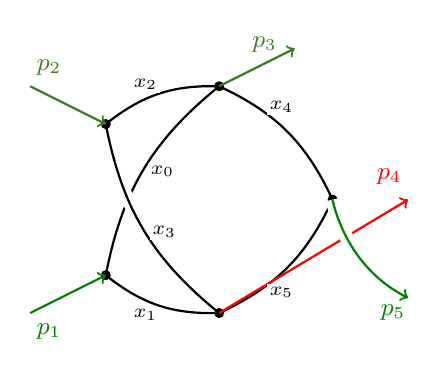
\begin{tikzpicture}[scale=.48]
 \coordinate (v1) at (2,3);
 \coordinate (v2) at (2,7);
 \coordinate (v3) at (5,8);
 \coordinate (v4) at (8,5);
 \coordinate (v5) at (5,2);

 \draw[hrf internal] (v3) to[bend right=20] (v1);
 \draw[hrf internal] (v3) to[bend right=20] (v2);
 \draw[white,double=white,double distance=3pt,thick]
   (v5) to[bend left=20] (v2);
 \draw[hrf internal] (v5) to[bend left=20] (v2);
 \draw[hrf internal] (v5) to[bend left=20] (v1);
 \draw[hrf internal] (v3) to[bend left=20] (v4);
 \draw[hrf internal] (v5) to[bend right=20] (v4);

 \foreach \v in {1,...,5} \node[hrf vertex] at (v\v) {};
 \draw[->,thick,Green] (0,2)--(v1);
 \draw[->,thick,OliveGreen] (0,8)--(v2);
 \draw[->,thick,OliveGreen] (v3)--(7,9);
 \draw[->,thick,red] (v5)--(10,5);
 \draw[white,line width=5pt]
   (v4) .. controls (8.2,4.1) and (8.8,3.0) .. (10,2.4);
 \draw[->,thick,Green]
   (v4) .. controls (8.2,4.1) and (8.8,3.0) .. (10,2.4);

 \node[hrf leg label,text=Green] at (.5,1.5) {$p_1$};
 \node[hrf leg label,text=OliveGreen] at (.5,8.5) {$p_2$};
 \node[hrf leg label,text=OliveGreen] at (6.2,9.1) {$p_3$};
 \node[hrf leg label,text=red] at (9.5,5.6) {$p_4$};
 \node[hrf leg label,text=Green] at (9.6,2.0) {$p_5$};

 \node[hrf edge label] at (3.50,5.75) {$x_0$};
 \node[hrf edge label] at (3.05,1.95) {$x_1$};
 \node[hrf edge label] at (3.05,8.05) {$x_2$};
 \node[hrf edge label] at (3.55,4.15) {$x_3$};
 \node[hrf edge label] at (6.65,7.45) {$x_4$};
 \node[hrf edge label] at (6.65,2.55) {$x_5$};
\end{tikzpicture}
\caption{The attachment used for the near-planar and representative
central-soft analyses.  The internal geometry is identical to
Fig.~\ref{fig:five-point-seed}, but \(p_4\) and \(p_5\) are interchanged.
The colours identify the corresponding external sectors without imposing
their geometric directions: \((p_2,p_3)\) are olive,
\((p_1,p_5)\) are green, and the central-soft momentum \(p_4\) is red.
The edge conventions are
\((x_0,\ldots,x_5)_{\rm here}=(x_1,\ldots,x_6)_{\rm Fig.\,3}\).}
\label{fig:five-point-near-planar-attachment}
\end{figure}

To expose the path symmetry, relabel the six edges as three two-edge paths
\((x_0,x_1)\), \((x_2,x_3)\) and \((x_4,x_5)\) between the two trivalent
endpoints, and put
\begin{equation}
 r_A=\frac{x_0}{x_1},\qquad r_B=\frac{x_2}{x_3},\qquad
 r_C=\frac{x_4}{x_5},\qquad
 \mathcal F=x_1x_3x_5\,\Phi(r_A,r_B,r_C).
 \label{eq:five-path-ratios}
\end{equation}
Here \(x_1,x_3,x_5>0\) are coordinates for the magnitudes on the three
two-edge paths, while \(r_A,r_B,r_C\) specify the ratios within them; they
are together six independent coordinates on the positive Schwinger
orthant.  Write
\begin{align}
 \Phi(\boldsymbol r)&=q_{AB}r_Ar_B+q_{BC}r_Br_C
 +q_{CA}r_Cr_A+b_A r_A+b_B r_B+b_C r_C
 =\frac12\boldsymbol r^T K\boldsymbol r+\boldsymbol b^T\boldsymbol r,
 \nonumber\\
 K&=\begin{pmatrix}
 0&q_{AB}&q_{CA}\\ q_{AB}&0&q_{BC}\\ q_{CA}&q_{BC}&0
 \end{pmatrix},
 \qquad \boldsymbol b=(b_A,b_B,b_C)^T.
 \label{eq:five-ratio-quadratic}
\end{align}
For the external attachment in Eq.~\eqref{eq:five-near-planar-attachment},
the entries are Mandelstam invariants, which may be expressed in terms of
the adjacent ones using five-point momentum conservation:
\begin{align}
 q_{AB}&=s_{35}=s_{12}-s_{34}-s_{45},
 &b_A&=s_{14}=-s_{15}+s_{23}-s_{45},\nonumber\\
 q_{BC}&=s_{13}=-s_{12}-s_{23}+s_{45},
 &b_B&=s_{24}=s_{15}-s_{23}-s_{34},\nonumber\\
 q_{CA}&=s_{23},
 &b_C&=s_{45}.
 \label{eq:five-ratio-coefficients}
\end{align}
Direct differentiation with respect to the ratios gives
\begin{equation}
 \nabla_{\boldsymbol r}\Phi=K\boldsymbol r+\boldsymbol b.
 \label{eq:five-ratio-gradient}
\end{equation}
The ratio-stationarity condition at \(\boldsymbol r=\boldsymbol\rho\) is
therefore the logically separate equation
\begin{equation}
 K\boldsymbol\rho=-\boldsymbol b.
 \label{eq:five-ratio-stationarity}
\end{equation}
The determinant of the coefficient matrix is
\begin{equation}
 \det K=2q_{AB}q_{BC}q_{CA}.
 \label{eq:five-ratio-determinant}
\end{equation}
Hence, whenever \(q_{AB}q_{BC}q_{CA}\ne0\), Eq.~\eqref{eq:five-ratio-stationarity}
determines a unique ratio vector
\(\boldsymbol\rho=(\rho_A,\rho_B,\rho_C)\).
Already at this generic kinematic point, define the three polynomials normal
to the ratio-stationary locus,
\begin{equation}
 f_A=x_0-\rho_Ax_1,\qquad f_B=x_2-\rho_Bx_3,
 \qquad f_C=x_4-\rho_Cx_5.
 \label{eq:five-path-normals}
\end{equation}
Here the \(\rho_I=-\left(K^{-1}\boldsymbol b\right)_I\) retain their full
kinematic dependence; no coplanar or MRK limit has yet been imposed.

Ratio stationarity is necessary but is not yet the complete Landau
condition.  To see the missing equation, use the independent path-magnitude
coordinates \(u_A=x_1\), \(u_B=x_3\), \(u_C=x_5\).  At fixed ratios,
\begin{equation}
 \mathcal F=u_Au_Bu_C\Phi,
 \qquad
 \frac{\partial\mathcal F}{\partial u_A}
 =u_Bu_C\Phi,
 \quad\text{and cyclically}.
 \label{eq:five-path-magnitude-equations}
\end{equation}
Since the path magnitudes are positive, stationarity in these directions
also requires
\begin{equation}
 \Phi(\boldsymbol\rho)=0.
 \label{eq:five-ratio-vanishing}
\end{equation}
In the original Schwinger parameters this condition follows automatically
from homogeneity once all derivative equations are imposed.  In the ratio
chart, however, \(\Phi\) contains both quadratic and linear terms and is not
homogeneous, so Eq.~\eqref{eq:five-ratio-vanishing} does not follow from
Eq.~\eqref{eq:five-ratio-stationarity}.  The stationary value follows
directly from Schur's formula for a bordered determinant.  Equation
\eqref{eq:five-ratio-stationarity} gives
\[
 \Phi(\boldsymbol\rho)
 =\frac12\boldsymbol b^T\boldsymbol\rho
 =-\frac12\boldsymbol b^TK^{-1}\boldsymbol b.
\]
For a block matrix, Schur's determinant formula is
\cite{Zhang:2005SchurComplement}
\[
 M=\begin{pmatrix}A&B\\ C&D\end{pmatrix},
 \qquad
 \det M=\det A\,\det\!\left(D-CA^{-1}B\right).
\]
Taking
\(M=\mathcal B\), \(A=K\), \(B=\boldsymbol b\),
\(C=\boldsymbol b^T\), and \(D=0\), one obtains
\[
 \mathcal B=\begin{pmatrix}K&\boldsymbol b\\
                  \boldsymbol b^T&0\end{pmatrix},
 \qquad
 \det\mathcal B
 =2\det K\,\Phi(\boldsymbol\rho)
 =4q_{AB}q_{BC}q_{CA}\,\Phi(\boldsymbol\rho).
\]
Using the Mandelstam identifications in
Eq.~\eqref{eq:five-ratio-coefficients}, five-point momentum conservation
gives
\(\det\mathcal B=\det(2p_i\!\cdot p_j)_{i,j=1}^{4}=\Gamma_5\).
Consequently,
\begin{equation}
 \Phi(\boldsymbol\rho)=
 \frac{\Gamma_5}{4q_{AB}q_{BC}q_{CA}}.
 \label{eq:five-stationary-gram}
\end{equation}
Completing the quadratic form about \(\boldsymbol\rho\), and then returning
to the original Schwinger parameters, gives the exact identity
\begin{align}
 \mathcal F={}&q_{AB}x_5f_Af_B+q_{BC}x_1f_Bf_C
 +q_{CA}x_3f_Cf_A
 +\frac{\Gamma_5}{4q_{AB}q_{BC}q_{CA}}x_1x_3x_5.
 \label{eq:five-full-stationary-decomposition}
\end{align}
This is an identity for the full massless \(\mathcal F\) at generic
five-point kinematics, not merely its restriction to the Gram surface.  It
makes direct contact with the HRF derivative strategy, but it is important
not to mistake this completed form for the algorithmic starting point.  HRF
starts from the usual Mandelstam representation of \(\mathcal F\).  For
example, direct differentiation there gives
\begin{equation}
 D_0\equiv\frac{\partial\mathcal F}{\partial x_0}
 =q_{AB}x_2x_5+q_{CA}x_3x_4+b_Ax_3x_5.
 \label{eq:five-raw-D0}
\end{equation}
Literal collection in \(q_{AB}\), \(q_{CA}\) and \(b_A\) exposes only
monomials.  The first component of \(K\boldsymbol\rho=-\boldsymbol b\),
\begin{equation}
 b_A=-q_{AB}\rho_B-q_{CA}\rho_C,
\end{equation}
instead reorganises the same derivative as
\begin{equation}
 D_0=q_{AB}x_5\bigl(x_2-\rho_Bx_3\bigr)
     +q_{CA}x_3\bigl(x_4-\rho_Cx_5\bigr)
 =q_{AB}x_5f_B+q_{CA}x_3f_C.
 \label{eq:five-adapted-D0}
\end{equation}
Thus the simple appearance of the \(f_I\) in the following equations has
already used the nontrivial stationary reorganisation.  In this example the
expansion has already been fixed at \(\Gamma_5=0\), and the complete leading
polynomial is the cancellation sector: \(\mathcal F_\star=\mathcal F_0=
\FSL\).  Candidate-specific saturation of its gradient ideal is therefore
legitimate and performs this reorganisation without assuming
\(\boldsymbol\rho\) in advance.  This special equality is precisely what
would fail for a generic starting polynomial containing an obstruction.
Since the final term of
Eq.~\eqref{eq:five-full-stationary-decomposition} is independent of
\(x_0,x_2,x_4\), the three stationary-adapted derivatives are
\begin{align}
 \frac{\partial\mathcal F}{\partial x_0}
 &=q_{AB}x_5f_B+q_{CA}x_3f_C,\nonumber\\
 \frac{\partial\mathcal F}{\partial x_2}
 &=q_{AB}x_5f_A+q_{BC}x_1f_C,\nonumber\\
 \frac{\partial\mathcal F}{\partial x_4}
 &=q_{BC}x_1f_B+q_{CA}x_3f_A.
 \label{eq:five-near-planar-gradient-system}
\end{align}
The determinant of this linear system in \((f_A,f_B,f_C)\) is
\(2q_{AB}q_{BC}q_{CA}x_1x_3x_5\).  Hence, in the interior positive orthant
and away from degenerate kinematics, these three derivative equations imply
\(f_A=f_B=f_C=0\).  The remaining derivatives then reduce to
\begin{equation}
 \left.\left(
 \frac{\partial\mathcal F}{\partial x_1},
 \frac{\partial\mathcal F}{\partial x_3},
 \frac{\partial\mathcal F}{\partial x_5}
 \right)\right|_{f_A=f_B=f_C=0}
 =\frac{\Gamma_5}{4q_{AB}q_{BC}q_{CA}}
 (x_3x_5,x_1x_5,x_1x_3).
 \label{eq:five-remaining-gradient-system}
\end{equation}
Likewise, Eq.~\eqref{eq:five-full-stationary-decomposition} restricted to
this locus equals
\(\Gamma_5x_1x_3x_5/(4q_{AB}q_{BC}q_{CA})\).  Thus the full derivative
system, viewed as a direct Landau analysis before choosing the expansion,
first exposes the candidate normal ideal
\(\langle f_A,f_B,f_C\rangle\), and its remaining equations then require
\(\Gamma_5=0\).  This explains why the near-planar expansion is required.
The HRF audit below starts only after that expansion has been fixed; on its
leading surface the saturation is therefore applied to \(\FSL\), not to a
generic obstructed starting polynomial.

Positivity of the resulting \(\rho_I\) is precisely the usual interior
first-sheet condition \(x_e>0\), because the \(\rho_I\) are the stationary
values of the positive ratios in Eq.~\eqref{eq:five-path-ratios}.  The
condition \(\Gamma_5=0\) is the coplanar boundary approached in the
near-planar limit, and it is also reached by the central-soft multi-Regge
limit discussed below.

This is the precise contrast with the Crown.  The Crown matrix \(K_C\) in
\eqref{eq:crown-ratio-quadratic} has a kinematics-independent zero mode, and
its stationary value vanishes throughout the generic wide-angle domain.
Here \(K\) is generically invertible: it fixes all three ratios, and the
remaining Landau equation restricts the kinematics to \(\Gamma_5=0\).
Only now specialise the generic construction to the near-planar expansion.
The normals become especially transparent in the exact chart
\eqref{eq:five-exact-kinematic-chart}.  On the coplanar boundary put
\begin{equation}
 \zeta=\bar\zeta=\xi,\qquad
 R=\frac{\xi+X_{45}(\xi+1)}
       {1+X_{34}X_{45}(\xi+1)}.
 \label{eq:five-near-planar-ratio-variables}
\end{equation}
The solution of \(K\boldsymbol\rho=-\boldsymbol b\) is then
\begin{equation}
 \rho_A=X_{34}\xi R,\qquad
 \rho_B=R,\qquad \rho_C=\xi,
 \label{eq:five-near-planar-rhos}
\end{equation}
and therefore
\begin{equation}
 f_A=x_0-X_{34}\xi R x_1,\qquad
 f_B=x_2-Rx_3,\qquad
 f_C=x_4-\xi x_5.
 \label{eq:five-near-planar-factors}
\end{equation}
On the physical positive-Landau branch
\(X_{34},X_{45},\xi>0\), so \(R>0\) and all three stationary ratios are
positive.  No MRK
hierarchy is used in these formulae.

To define the near-planar expansion, let \(\boldsymbol{\kappa}\) denote four
coordinates tangent to the Gram surface and use \(\Gamma_5\) as a local
normal coordinate.  Then
\begin{equation}
 \mathcal F(\Gamma_5,\boldsymbol{\kappa})
 =\mathcal F_0(\boldsymbol{\kappa})
  +\Gamma_5\mathcal F_{\Gamma_5}(\boldsymbol{\kappa})
  +O(\Gamma_5^2).
 \label{eq:five-gram-expansion}
\end{equation}
There is no conflict between the apparently nonlinear kinematic dependence
in Eq.~\eqref{eq:five-full-stationary-decomposition} and the linearity of
\(\mathcal F\) in Mandelstam invariants.  The Gram determinant \(\Gamma_5\)
is itself a nonlinear polynomial in those invariants.  Replacing one
Mandelstam variable by \(\Gamma_5\) is therefore a nonlinear change of
kinematic coordinates, and at fixed \(\boldsymbol\kappa\)
\begin{equation}
 \mathcal F_{\Gamma_5}
 =\left.\frac{\partial\mathcal F}{\partial\Gamma_5}
  \right|_{\boldsymbol\kappa}
 =\sum_a\frac{\partial\mathcal F}{\partial s_a}
  \left.\frac{\partial s_a}{\partial\Gamma_5}
  \right|_{\boldsymbol\kappa}.
 \label{eq:five-gram-chain-rule}
\end{equation}
The Jacobian factors on the right need not be linear functions of the
remaining kinematics.  Equivalently, the separate terms in
Eq.~\eqref{eq:five-full-stationary-decomposition} contain the rational
ratios \(\boldsymbol\rho=-K^{-1}\boldsymbol b\); their nonlinear dependence
cancels in the sum, restoring the original Mandelstam-linear polynomial.

The complete coefficient \(\mathcal F_{\Gamma_5}\) away from the stationary
locus depends on the choice of the tangent coordinates
\(\boldsymbol\kappa\).  Its restriction to \(f_A=f_B=f_C=0\), however, is
fixed by Eq.~\eqref{eq:five-full-stationary-decomposition}:
\begin{equation}
 \left.\mathcal F_{\Gamma_5}\right|_{f_A=f_B=f_C=0}
 =\frac{x_1x_3x_5}{4q_{AB}q_{BC}q_{CA}}.
 \label{eq:five-gram-coefficient-on-locus}
\end{equation}
This stationary contribution is not an
``obstruction'' in the technical HRF sense: it is absent from the leading
polynomial by the definition of the chosen kinematic expansion, rather than
being made subleading by the HR scaling.  Since
\(\Gamma_5=O(\lambda^2)\), this contribution first appears two powers beyond
\(\mathcal F_0\).  Its precise weight relative to the cancelled leading
sector and to \(\mathcal U\) will follow only after the region vector has
been determined below.  The leading polynomial itself has the symmetric
factorised form
\begin{equation}
 \mathcal F_0\equiv\left.\mathcal F\right|_{\Gamma_5=0}
 =q_{AB}x_5f_Af_B+q_{BC}x_1f_Bf_C+q_{CA}x_3f_Cf_A.
 \label{eq:five-coplanar-factorisation}
\end{equation}
Thus the HR generators are the factorised products
\(f_Af_B,f_Bf_C,f_Cf_A\), not the individual normal equations.  This is a
three-generator ideal and is more general than the pair-sector search used
in the earlier examples.

Using Eq.~\eqref{eq:five-ratio-coefficients}, the outer coefficients in these
six summands are the distinct invariant sectors
\(q_{AB}=s_{35}\), \(q_{BC}=s_{13}\) and \(q_{CA}=s_{23}\).  If the
stationary-adapted derivatives in
Eq.~\eqref{eq:five-near-planar-gradient-system} have been obtained, their
sector-decomposed form exposes the normals directly, up to positive monomial
factors:
for example the two sectors of the first line expose \(f_B\) and \(f_C\),
and the remaining lines expose all three \(f_I\).  In the Crown this form is
available by direct invariant-sector harvesting.  Here the \(f_I\) contain
kinematic stationary ratios, so the corresponding reorganisation must first
be derived.  The full Landau analysis above first shows that the remaining
equations require \(\Gamma_5=0\).  Once the expansion has been fixed on that
surface, saturation by the nonzero determinant following
Eq.~\eqref{eq:five-near-planar-gradient-system} is candidate-specific and
the ideal generated by these three leading-sector derivatives is precisely
\(\langle f_A,f_B,f_C\rangle\).  It therefore recovers the three normals
without assuming them in advance.  Factoring each derivative separately
cannot do so in general, because an individual derivative is a linear
combination of two normals rather than a multiple of either one.  Substitution
into \(\mathcal F_0\) then identifies the HR generator ideal
\(\langle f_Af_B,f_Bf_C,f_Cf_A\rangle\).

For the expansion defined in Eqs.~\eqref{eq:five-near-planar-chart} and
\eqref{eq:five-near-planar-limit}, the certified original-coordinate vector
and weights are
\begin{equation}
 \vHR=(-2,-2,-2,-2,-2,-2;1),
 \qquad (\WSL,\WHR)=(-6,-4).
 \label{eq:five-near-planar-vector}
\end{equation}
The comparison announced above is now fixed.  Every cubic monomial in
\(\mathcal F_0\) has raw weight \(-6\).  The normal factor
\(\Gamma_5=O(\lambda^2)\) raises the weight of
\(\Gamma_5\mathcal F_{\Gamma_5}\) to \(-4\), while the quadratic polynomial
\(\mathcal U\) also has weight \(-4\).  Cancellation on the singular locus
promotes \(\mathcal F_0\) from \(\WSL=-6\) to the same resolved weight
\(\WHR=-4\).  Thus the cancelled leading sector, the first Gram-normal
correction and \(\mathcal U\) all enter the resolved LP polynomial at
\(\WHR\).
The dissection coordinates can be stated explicitly.  Take the tangential
path magnitudes \(u_A=x_1\), \(u_B=x_3\), \(u_C=x_5\) and the three normals
\(y_I=f_I\) of Eq.~\eqref{eq:five-path-normals}.  In a sign sector put
\[
 \begin{array}{lll}
 x_0=\rho_Au_A+\sigma_A t_A,&x_1=u_A,&t_A=|y_A|,\\
 x_2=\rho_Bu_B+\sigma_B t_B,&x_3=u_B,&t_B=|y_B|,\\
 x_4=\rho_Cu_C+\sigma_C t_C,&x_5=u_C,&t_C=|y_C|,
 \end{array}
 \qquad \sigma_I=\pm1 .
\]
At fixed kinematics this transformation has unit absolute Jacobian.  The
ordinary lower facet in these local coordinates has
\(u_I\sim\lambda^{-2}\) and \(t_I\sim\lambda^{-1}\), and its pullback is
Eq.~\eqref{eq:five-near-planar-vector}.

First perform the power count entirely in parameter space and in the
original variables.  Without the cancellation restriction, six measures
with \(x_e\sim\lambda^{-2}\) would give \(\lambda^{-12}\).  For each pair,
however, only a relative neighbourhood
\(|f_I|=O(\lambda^{-1})\) contributes, rather than the
natural width \(O(\lambda^{-2})\).  The three restrictions restore one power
of \(\lambda\) each.  Equivalently, the dissected measure contains three
\(u_I\) and three \(t_I\) integrations.  Since the resolved LP polynomial
has weight \(-4\),
\begin{align}
 I_{\rm par}^{\rm scalar}
 &\sim
 \underbrace{\lambda^{-12}}_{\text{unrestricted}}
 \;\underbrace{\lambda^{3}}_{\text{restricted widths}}
 \;\underbrace{\bigl(\lambda^{-4}\bigr)^{-D/2}}_{\mathcal P^{-D/2}}
 \nonumber\\
 &=
 \underbrace{(\lambda^{-2})^3(\lambda^{-1})^3}
             _{\prod_I\dd u_I\,\dd t_I\ \text{after dissection}}
 \bigl(\lambda^{-4}\bigr)^{-D/2}
 =\lambda^{2D-9}=\lambda^{-1-4\epsilon},
 \qquad D=4-2\epsilon.
 \label{eq:five-near-planar-parameter-power}
\end{align}

The momentum-space count is independent.  Choose two path momenta, say
\(q_A\) and \(q_B\), as the loop variables; momentum conservation fixes
\(q_C=-p_3-q_A-q_B\).  Each unrestricted collinear loop measure scales as
\(\lambda^D\): the momentum fraction has width \(O(1)\), its conjugate
light-cone component has width \(O(\lambda^2)\), and the \(D-2\) transverse
components each have width \(O(\lambda)\).  Keeping the dependent momentum
\(q_C\) collinear to its wide-angle direction further confines
\(\delta\xi_A\) and \(\delta\xi_B\) to widths \(O(\lambda)\) and
\(O(\lambda^2)\), giving the additional \(\lambda^3\).  All six propagator virtualities are
\(q_e^2=O(\lambda^2)\).  Therefore
\begin{equation}
 I_{\rm mom}^{\rm scalar}
 \sim
 \underbrace{(\lambda^D)^2}_{\text{collinear measures}}
 \;\underbrace{\lambda^3}_{\text{restricted support}}
 \;\underbrace{(\lambda^{-2})^6}_{\text{propagators}}
 =\lambda^{2D-9}=\lambda^{-1-4\epsilon}.
 \label{eq:five-near-planar-momentum-power}
\end{equation}
The agreement of Eqs.~\eqref{eq:five-near-planar-parameter-power} and
\eqref{eq:five-near-planar-momentum-power} checks both the cancellation
depth in the original Schwinger domain and its translation into restricted
loop-momentum support.

\subsubsection{Central-soft MRK: the full-layer certificate}
\label{sec:five-point-central-soft-status}

Starting again from the generic chart
\eqref{eq:five-exact-kinematic-chart}--\eqref{eq:five-zeta-chart}, keep the
two MRK rapidity gaps large while scaling all components of the central
momentum as \(p_4^\mu=O(\delta^a)\), with the rapidity parameter
\(x_{\rm MRK}=O(\delta^b)\) and \(0<a<b\).  The same exact variables used
above define this path by
\begin{align}
 \zeta&=\widehat\zeta\,\delta^a,&
 \bar\zeta&=\widehat{\bar\zeta}\,\delta^a,&
 Q_4^2&=\widehat Q_4^2\delta^{2a},\nonumber\\
 X_{34}&=\widehat X_{34}\delta^{-(a+b)},&
 X_{45}&=
 \frac{\widehat X_{45}\delta^{a-b}}
 {(1+\widehat\zeta\delta^a)
  (1+\widehat{\bar\zeta}\delta^a)}.
 \label{eq:five-central-soft-common-path}
\end{align}
All hatted quantities are fixed and nonzero.  In the physical region
\(\widehat{\bar\zeta}=\widehat\zeta^*\); the denominator in \(X_{45}\)
keeps the path exactly on shell rather than specifying only its leading
valuation.  In this chart,
\begin{equation}
 \epsilon_5=s_{12}Q_4^2
 \frac{\zeta-\bar\zeta}{\zeta\bar\zeta}.
 \label{eq:five-central-soft-gram}
\end{equation}
Near-planar wide-angle scattering sends \(\zeta-\bar\zeta\to0\) at fixed
\(Q_4^2\), whereas central-soft MRK sends
\(Q_4^2\to0\) and \(\zeta,\bar\zeta\to0\) together.  Both reach a normalized
planar boundary, but this kinematic relation does not imply the same HR.

For reference, the earlier executable audit used finite positive
coefficients \(P,K,M,R,T\) and a transverse coefficient \(C\).  It is
exactly the same path under
\begin{equation}
 \widehat Q_4^2=R,\qquad
 \widehat X_{34}=\frac PK,\qquad
 \widehat X_{45}=\frac{KM}{T},\qquad
 \widehat\zeta\widehat{\bar\zeta}=\frac RT,\qquad
 \widehat\zeta+\widehat{\bar\zeta}=\frac{\sigma C}{T}.
 \label{eq:five-central-soft-old-chart-map}
\end{equation}
This map is used only as an exact equivalence and positivity audit below;
the common variables in Eq.~\eqref{eq:five-central-soft-common-path} define
the expansion.

For the representative central-soft attachment and \((a,b)=(1,2)\), the
alignment face gives
\begin{align}
 \boldsymbol\phi&=(-3,-3,0,-3,-3,-3),\nonumber\\
 \mathcal F_{-10}^{\rm align}
 &=-\frac{\widehat X_{45}\widehat Q_4^2}
 {\widehat\zeta\widehat{\bar\zeta}}
 (\widehat X_{34}x_2-x_3)(x_1x_4-x_0x_5).
 \label{eq:five-central-soft-face}
\end{align}
The relative HRF vector is uniform,
\begin{equation}
 \boldsymbol\rho=(-1,-1,-1,-1,-1,-1),
 \qquad
 \widetilde{\boldsymbol v}^{\rm CS}=(-4,-4,-1,-4,-4,-4).
 \label{eq:five-central-soft-vector}
\end{equation}
The exact chart is Laurent in \(\delta\).  Factoring out the growing hard
invariant \(s_{12}\) implements the dimensionless normalization in which
Eq.~\eqref{eq:five-central-soft-vector} is the infrared HRF vector, and
\begin{equation}
 \vHR^{\rm CS}=(-4,-4,-1,-4,-4,-4;1),
 \qquad (\WSL,\WHR)=(-9,-8).
 \label{eq:five-central-soft-physical-vector}
\end{equation}
Adding \(+4\) uniformly converts to dimensionful Schwinger parameters while
\(s_{12}\sim\delta^{-4}\) itself varies, but the resulting non-negative list
is a change of hard-scale units, not the infrared region vector.
The next layer contains
\begin{equation}
 -\frac{\widehat Q_4^2}
 {\widehat\zeta\widehat{\bar\zeta}}x_0x_3x_4,
 \label{eq:five-central-soft-physical-F}
\end{equation}
which remains nonzero on the two-factor locus and has weight \(-8\), exactly
the leading \(\mathcal U\) weight.  In the representative labeling,
\begin{equation}
 \mathcal U_{-8}=x_0x_3+x_1x_3+x_0x_4+x_1x_4+x_3x_4
                 +x_0x_5+x_1x_5+x_3x_5.
 \label{eq:five-central-soft-U}
\end{equation}
Thus Eq.~\eqref{eq:five-central-soft-physical-F} is not an obstruction below
the physical layer; it is part of that layer.  Together with the promoted
factorised terms, the resolved support has affine rank six and the unique
inward normal is precisely
Eq.~\eqref{eq:five-central-soft-physical-vector}.  The hierarchy gap is one.

The result is stable for the tested rates \((a,b)=(1,2),(1,3),(2,3)\) and
for both transverse-sign charts.  Among the twelve inequivalent external
attachments of the fixed topology, exactly six have this certificate:
those in which the central gluon is attached to either four-valent internal
vertex.  The other six have no staged candidate.  For each positive
attachment two additional staged presentations fail the final lower-facet
test, so the accepted count is one rather than three.

The reason is already visible on the leading face exposed by the natural
alignment vector \(\boldsymbol\phi=(-3,-3,0,-3,-3,-3)\).  If the soft
particle \(p_4\) is emitted from the trivalent middle vertex \(4\), the
aligned face is
\begin{equation}
 \mathcal F_{\rm mid}^{\rm align}
 =-\frac{\widehat X_{45}\widehat Q_4^2}
 {\widehat\zeta\widehat{\bar\zeta}}x_1
 \big[(\widehat X_{34}x_2-x_3)x_4
       +\widehat X_{34}x_2x_5\big].
 \label{eq:five-central-soft-middle-attachment}
\end{equation}
The bracket can vanish for positive parameters, but the zero is not
stationary:
\begin{equation}
 \frac{\partial}{\partial x_5}
 \big[(\widehat X_{34}x_2-x_3)x_4
       +\widehat X_{34}x_2x_5\big]
 =\widehat X_{34}x_2>0.
 \label{eq:five-central-soft-middle-derivative}
\end{equation}
The unmatched term \(\widehat X_{34}x_2x_5\) records that the soft leg has selected the
middle of one particular theta path.

If \(p_4\) is attached instead to the four-valent theta endpoint \(5\), the
corresponding face factorises,
\begin{equation}
 \mathcal F_{\rm end}^{\rm align}
 =-\frac{\widehat X_{45}\widehat Q_4^2}
 {\widehat\zeta\widehat{\bar\zeta}}
 (\widehat X_{34}x_2-x_3)(x_1x_4-x_0x_5).
 \label{eq:five-central-soft-end-attachment}
\end{equation}
The two factors are independent routing differences.  Their simultaneous
zero is stationary because \(d(AB)=B\,dA+A\,dB\).  At the endpoint all
three theta paths remain available, allowing two independent
rebalancings of the two-loop flow.  Emission in the middle of one path
distinguishes that path and prevents the second rebalancing.  The full
twelve-attachment scan confirms that no alternative aligned face restores
a pinch for a trivalent attachment.

For the scalar power count define the local normals
\begin{equation}
 A=x_2-\widehat X_{34}^{-1}\delta^3x_3,
 \qquad B=x_1x_4-x_0x_5.
 \label{eq:five-central-soft-local-normals}
\end{equation}
Their generic weights are \(-1\) and \(-8\), respectively, and the HRF gap
restricts \(A\) to weight \(0\).  Four tangential coordinates contribute
\(-16\).  Solving for \(x_2,x_5\) gives the Jacobian
\(-1/x_0\), of weight \(+4\).  The parameter-space measure therefore
contributes \(\delta^{-20}\), while the resolved LP weight \(-8\) gives
\(\mathcal P^{-D/2}\sim\delta^{4D}\).

In momentum space choose \(r=q_0\) and \(\ell=q_0-q_4\).  A complete edge
assignment is
\begin{equation}
\begin{array}{c|cccccc}
e&0&1&2&3&4&5\\ \hline
(q_e^+,q_e^-,|q_{e\perp}|)&
(4,0,2)&(4,0,2)&(0,1,2)&(3,1,2)&(4,0,2)&(4,0,2)\\
q_e^2&4&4&1&4&4&4
\end{array}
\label{eq:five-central-soft-edge-powers}
\end{equation}
where the entries are powers of \(\delta\) in hard-scale-normalized
momenta.  The \(q_0,q_1\) poles pinch \(r^+\) with width \(\delta^4\);
\(q_4,q_5\) pinch \(\ell^+\) with width \(\delta^4\); and \(q_2,q_3\)
pinch \(\ell^-\) with width \(\delta\).  Both transverse widths scale as
\(\delta^2\).  Hence the loop widths are \((4,0,2)\) and \((4,1,2)\),
giving measure power \(4D+1\).  The denominator powers sum to \(21\).
The two representations agree:
\begin{equation}
 I_{\rm CS}^{\rm scalar}\sim
 \underbrace{\delta^{-20}\delta^{4D}}_{\text{parameter space}}
 =\underbrace{\delta^{4D+1}\delta^{-21}}_{\text{momentum space}}
 =\delta^{4D-20}
 =\delta^{-4-8\epsilon},\qquad D=4-2\epsilon.
 \label{eq:five-central-soft-power}
\end{equation}
This is the reduced integral with \(s_{12}\) factored out, which is the
appropriate convention for diagnosing an infrared region.  Restoring the
engineering-dimension factor \(s_{12}^{D-6}\), with
\(s_{12}\sim\delta^{-4}\), is a separate overall conversion and must not be
used to redefine the HRF vector.

\iffalse
The two five-point regions nevertheless have an algebraic relation.  In the
central-soft degeneration (\rho_A=\rho_C), so
\begin{equation}
 x_1x_4-x_0x_5=x_1f_C-x_5f_A,\qquad
 Px_2-Kx_3=P f_B.
 \label{eq:five-region-ideal-relation}
\end{equation}
Their product lies in the near-planar ideal generated by (f_Af_B) and
(f_Bf_C); the third generator (f_Af_C) is suppressed on the selected
MRK face.  Thus the two limits expose a common path-normal geometry of the
same seed topology, but they are not the same region: their physical vectors,
momentum modes and scalar powers are different.
\fi

The limiting algebraic structures of the two regions nevertheless have a
relation; this comparison does not construct either limit as a sublimit of
the other.  On the aligned central-soft face the two corresponding path
ratios coincide, which may be written \(\rho_A=\rho_C\), so
\begin{equation}
 x_1x_4-x_0x_5=x_1f_C-x_5f_A,\qquad
 \widehat X_{34}x_2-x_3=\widehat X_{34}f_B.
 \label{eq:five-region-ideal-relation-clean}
\end{equation}
Their product lies in the near-planar ideal generated by \(f_Af_B\) and
\(f_Bf_C\); the third generator \(f_Af_C\) is suppressed on the selected
MRK face.  Thus the two limits expose a common path-normal geometry of the
same seed topology, but they are not the same region: their physical vectors,
momentum modes and scalar powers are different.

\iffalse
\subsubsection{Central-soft five-point multi-Regge kinematics}
\label{sec:five-point-central-soft-mrk}

We now keep the multi-Regge rapidity ordering but approach the additional
surface on which the central emitted momentum becomes soft.  Use the
all-outgoing convention
\begin{equation}
 -p_1-p_2+p_3+p_4+p_5=0,
 \label{eq:five-mrk-process}
\end{equation}
so that \(p_1,p_2\) are incoming and \(p_3,p_4,p_5\) are ordered from forward
to backward rapidity.  Let \(0<a<b\) and choose the exact on-shell chart
\begin{align}
 p_3^+&=P\delta^{-b},&
 p_3^-&=\frac{T}{P}\delta^b,&
 \boldsymbol p_{3\perp}&=\boldsymbol q,
 \nonumber\\
 p_4^+&=K\delta^a,&
 p_4^-&=\frac{R}{K}\delta^a,&
 \boldsymbol p_{4\perp}&=\delta^a\boldsymbol k,
 \nonumber\\
 p_5^-&=M\delta^{-b},&
 p_5^+&=\frac{T+\sigma C\delta^a+R\delta^{2a}}{M}\delta^b,&
 \boldsymbol p_{5\perp}&=-\boldsymbol q-\delta^a\boldsymbol k,
 \label{eq:five-mrk-chart}
\end{align}
where
\begin{equation}
 T=|\boldsymbol q|^2,\qquad R=|\boldsymbol k|^2,\qquad
 2\operatorname{Re}(\boldsymbol q\overline{\boldsymbol k})=\sigma C,
 \qquad C^2<4RT,
 \label{eq:five-mrk-domain}
\end{equation}
and \(P,M,K,R,T,C>0\), \(\sigma=\pm1\).  The incoming components are fixed by
Eq.~\eqref{eq:five-mrk-process}, so on-shellness and momentum conservation
hold at every nonzero \(\delta\), not only at leading power.

The rapidities obey
\begin{equation}
 y_3\sim-b\log\delta,\qquad y_4=O(1),\qquad
 y_5\sim b\log\delta,
 \label{eq:five-mrk-rapidities}
\end{equation}
while all components of \(p_4\) scale as \(\delta^a\).  Thus the rapidity
hierarchy of MRK is preserved, but the usual assumption of comparable
transverse momenta is not: this is a composite central-soft MRK limit.
For the representative path \((a,b)=(1,2)\),
\begin{align}
 s_{12}&=PM\delta^{-4}+O(\delta^{-1}),&
 s_{34}&=\frac{PR}{K}\delta^{-1}+O(\delta),&
 s_{45}&=KM\delta^{-1}+O(\delta),
 \nonumber\\
 s_{23}&=-T+O(\delta^3),&
 s_{15}&=-T-\sigma C\delta-R\delta^2+O(\delta^3).
 \label{eq:five-mrk-invariants}
\end{align}
This has the physical signs \(s_{12},s_{34},s_{45}>0\) and
\(s_{23},s_{15}<0\).  In ordinary five-point MRK the central transverse
momentum remains finite; the HR described below is absent in that expansion.

\paragraph{Central-soft MRK certificate for the seed.}

The internal edges are again those of Eq.~\eqref{eq:five-edges}.  To match
the MRK computation we relabel them as
\begin{equation}
 \{(1,3),(1,5),(2,3),(2,5),(3,4),(4,5)\}
 \longleftrightarrow(x_0,\ldots,x_5),
 \label{eq:five-mrk-edges}
\end{equation}
and use the representative attachment
\begin{equation}
 p_1\to1,\quad p_2\to2,\quad p_3\to3,\quad
 p_5\to4,\quad p_4\to5.
 \label{eq:five-mrk-attachments}
\end{equation}
This is precisely the attachment drawn in
Fig.~\ref{fig:five-point-near-planar-attachment}: the central gluon is
attached to a four-valent internal vertex.  A scan of the twelve
inequivalent external attachments finds an HR
for precisely the six in which \(p_4\) is attached to either of the two
four-valent vertices.  All twelve one-loop pentagons are negative, and the
same two-loop attachments are negative in generic MRK.  The result is
unchanged for \((a,b)=(1,2),(1,3),(2,3)\) and for both signs \(\sigma\).

The origin of this attachment dependence is already visible before the
full lower-facet test.  Apply the natural alignment vector
\(\boldsymbol\phi=(-3,-3,0,-3,-3,-3)\) to the two attachments.  If the
soft particle \(p_4\) is emitted from the trivalent middle vertex \(4\), the
leading face is
\begin{equation}
 \mathcal F_{\rm mid}^{\rm align}
 =-Mx_1\big[(Px_2-Kx_3)x_4+Px_2x_5\big].
 \label{eq:five-mrk-middle-attachment-face}
\end{equation}
The bracket can vanish for positive parameters, but it cannot be a positive
Landau pinch: its derivative with respect to \(x_5\) is \(Px_2>0\).
Equivalently, on the zero of the bracket,
\(\partial\mathcal F_{\rm mid}^{\rm align}/\partial x_5=-MPx_1x_2\ne0\).
The term \(Px_2x_5\) is an unmatched contribution from the single theta
path on which the soft leg is inserted.

When \(p_4\) is instead attached to the four-valent theta endpoint \(5\),
the corresponding face becomes
\begin{equation}
 \mathcal F_{\rm end}^{\rm align}
 =-M(Px_2-Kx_3)(x_1x_4-x_0x_5).
 \label{eq:five-mrk-endpoint-attachment-face}
\end{equation}
It contains two independent routing differences.  On their simultaneous
zero every derivative of the product vanishes, because
\(d(AB)=B\,dA+A\,dB\).  Topologically, injection at a theta endpoint leaves
three alternative internal paths available and permits the two-loop flow to
rebalance in two independent ways.  Injection in the middle of one path
distinguishes that path and leaves the unmatched term in
Eq.~\eqref{eq:five-mrk-middle-attachment-face}.  The complete twelve-attachment
scan confirms that no different aligned face restores a pinch for a
trivalent attachment.

For Eq.~\eqref{eq:five-mrk-attachments}, asymptotic-order alignment gives
\begin{equation}
 \boldsymbol\phi=(-3,-3,0,-3,-3,-3).
 \label{eq:five-mrk-alignment-vector}
\end{equation}
On the exposed face the superleading polynomial factorises as
\begin{equation}
 \mathcal F_\star^{\rm MRK}
 =\SLcolour{KM^2P\,(Kx_3-Px_2)(x_1x_4-x_0x_5)},
 \qquad \FObs=0,
 \label{eq:five-mrk-aligned-polynomial}
\end{equation}
up to an irrelevant overall sign.  Its positive cancellation locus is
\begin{equation}
 Px_2-Kx_3=0,\qquad x_1x_4-x_0x_5=0.
 \label{eq:five-mrk-cancellation-locus}
\end{equation}
The second-stage HRF vector in the aligned coordinates is uniform,
\begin{equation}
 \boldsymbol\rho=(-1,-1,-1,-1,-1,-1),
 \label{eq:five-mrk-second-vector}
\end{equation}
and Eq.~\eqref{eq:alignment-composition} gives the total vector
\begin{equation}
 \vHR^{\rm MRK}=(-4,-4,-1,-4,-4,-4;1).
 \label{eq:five-mrk-total-vector}
\end{equation}
The final aligned HRF step has gap one.  For absolute counting in the
original exact chart, however, the raw superleading layer has weight \(-13\)
and the resolved scaleful LP layer has weight \(-8\).  The full cancellation
depth is therefore five: four powers are exposed by alignment and one by the
final HRF step.  Quoting only the latter would lose essential information.

\paragraph{Complete edge flow and mode-adapted loop basis.}

The full valuation-level solution is shown in
Table~\ref{tab:five-mrk-edge-flow}.  Here \(q_e\) denotes the momentum on the
edge carrying \(x_e\) in Eq.~\eqref{eq:five-mrk-edges}.  ``Enhanced'' means
that the displayed components would give a lower virtuality power unless
their leading longitudinal and transverse contributions cancel.
\begin{table}[H]
\centering
\small
\begin{tabular}{@{}c c c l@{}}
\toprule
edge & \((a_e,b_e,c_e)\) & \(q_e^2\) & realization\\
\midrule
\(q_0\) & \((6,-2,2)\) & \(\delta^4\) & balanced\\
\(q_1\) & \((6,-2,2)\) & \(\delta^4\) & balanced\\
\(q_2\) & \((-2,3,2)\) & \(\delta\) & longitudinal dominated\\
\(q_3\) & \((1,3,2)\) & \(\delta^4\) & balanced\\
\(q_4\) & \((2,-2,0)\) & \(\delta^4\) & enhanced\\
\(q_5\) & \((4,-2,1)\) & \(\delta^4\) & enhanced\\
\bottomrule
\end{tabular}
\caption{Complete edge-momentum valuations for the central-soft MRK HR.
The table satisfies the target virtualities and tropical vertex conservation.
The pole analysis below supplies the additional local widths required for a
mode-complete solution.}
\label{tab:five-mrk-edge-flow}
\end{table}

The edge momenta \(q_0\) and \(q_3\) form one convenient chord basis, but
their central edge powers are not the local widths of a mode-adapted basis.
Set
\begin{equation}
 r=q_0,\qquad \ell=q_0-q_4.
 \label{eq:five-mrk-glauber-rerouting}
\end{equation}
Momentum conservation then gives
\begin{equation}
 q_2=p_3-\ell,\qquad q_3=\ell+p_2-p_3,
 \qquad q_4=r-\ell,\qquad q_5=p_5-r+\ell.
 \label{eq:five-mrk-mode-routing}
\end{equation}
The central value is
\begin{equation}
 \ell\big|_{\rm pinch}\sim(\delta^2,\delta^2,1),
 \label{eq:five-mrk-glauber-value}
\end{equation}
but its local integration widths are more restrictive.

Four denominators depend algebraically on \(\ell^+\).  For \(q_2\) and
\(q_3\), however, the coefficient is of order \(\delta^3\).  A local
\(\Delta\ell^+\sim\delta^6\) fluctuation enters them only at order
\(\delta^9\), subleading relative to their virtualities \(\delta\) and
\(\delta^4\).  The two leading-sensitive denominators are instead
\begin{align}
 D_4={}&(r^+-\ell^+)(r^--\ell^-)
       -|r_\perp-\ell_\perp|^2+i0,
 \label{eq:five-mrk-D4}\\
 D_5={}&(p_5^+-r^++\ell^+)(p_5^--r^-+\ell^-)
       -|p_{5\perp}-r_\perp+\ell_\perp|^2+i0.
 \label{eq:five-mrk-D5}
\end{align}
Writing \(q_4^-=r^--\ell^-\) and
\(q_5^-=p_5^--r^-+\ell^-\), their poles are
\begin{align}
 \ell_4^+={}&r^+-\frac{|q_{4\perp}|^2}{q_4^-}
              +\frac{i0}{q_4^-},
 \label{eq:five-mrk-pole4}\\
 \ell_5^+={}&r^+-p_5^++\frac{|q_{5\perp}|^2}{q_5^-}
              -\frac{i0}{q_5^-}.
 \label{eq:five-mrk-pole5}
\end{align}
On the physical positive-flow branch \(q_4^-,q_5^->0\), the first pole is
above and the second below the real axis.  Both slopes have power \(-2\),
whereas \(D_4,D_5\sim\delta^4\).  Equations
\eqref{eq:light-cone-pole-rule}--\eqref{eq:light-cone-pinch-width} therefore
give
\begin{equation}
 \Delta\ell^+\sim\delta^6.
 \label{eq:five-mrk-ellplus-width}
\end{equation}
The residual relation \(q_2=p_3-\ell\) fixes
\(\Delta\ell^-\sim\delta^3\) and
\(\Delta\ell_\perp\sim\delta^2\).  Thus
\begin{equation}
 \ell:\quad (\Delta\ell^+,\Delta\ell^-,
                   |\Delta\ell_\perp|)
       \sim(\delta^6,\delta^3,\delta^2).
 \label{eq:five-mrk-glauber-widths}
\end{equation}
Since \(6+3>2\times2\), \(\ell\) is one genuine Glauber integration mode.
There are not two Glauber loops.  The other independent variable has local
widths \(r\sim(\delta^6,\delta^{-2},\delta^2)\).  Its plus-component width
is independently confirmed by the \(q_0\) and \(q_1=p_1-r\) poles, which
also approach from opposite half-planes and give
\(\Delta r^+\sim\delta^6\).

\paragraph{Parameter- and momentum-space power counting.}

The sum of the six edge exponents in
Eq.~\eqref{eq:five-mrk-total-vector} is \(-21\).  Restriction to the
simultaneous cancellation neighbourhood restores five powers, giving the
effective parameter-measure weight \(-16\).  Since the resolved LP weight is
\(-8\),
\begin{equation}
 I_{\rm MRK}^{\rm scalar}\sim
 \delta^{-21+5}\bigl(\delta^{-8}\bigr)^{-D/2}
 =\delta^{4D-16}=\delta^{-8\epsilon}.
 \label{eq:five-mrk-parameter-power}
\end{equation}
The unit-numerator scalar HR is therefore leading power at \(D=4\), with the
nontrivial \(\epsilon\)-dependence expected of an infrared region.

The pole analysis now gives an independent momentum-space count.  The
\(r\) measure has power
\(6-2+2(D-2)=2D\), while the Glauber measure has power
\(6+3+2(D-2)=2D+5\).  The virtuality powers in
Table~\ref{tab:five-mrk-edge-flow} sum to 21.  Hence
\begin{equation}
 \frac{\dd^D\ell_1\,\dd^D\ell_2}
      {\prod_{e=0}^{5}q_e^2}
 \sim\delta^{,2D+(2D+5)-21}
 =\delta^{4D-16}=\delta^{-8\epsilon}.
 \label{eq:five-mrk-momentum-power}
\end{equation}
This agrees with Eq.~\eqref{eq:five-mrk-parameter-power}.  No separate
five-power cancellation-depth correction is inserted in momentum space: the
restricted support is already encoded in the local widths, most visibly in
\(\Delta\ell^+\sim\delta^6\).  Treating the central powers of \((q_0,q_3)\)
as integration widths and then adding the cancellation depth would double
count the restriction.

\fi
\subsubsection{Comparison of the certified five-point regions}

\begin{center}
\small
\begin{tabular}{@{}
 >{\raggedright\arraybackslash}p{0.20\textwidth}
 >{\centering\arraybackslash}p{0.29\textwidth}
 >{\centering\arraybackslash}p{0.16\textwidth}
 >{\raggedright\arraybackslash}p{0.23\textwidth}@{}}
\toprule
Expansion & total edge vector & scalar power & momentum signature\\
\midrule
Spacelike collinear &
\((-2,-1,-2,-2,-2,-1;1)\) &
\(\delta^{-1-4\epsilon}\) &
soft \(+\) Glauber\\
Near-planar wide angle &
\((-2,-2,-2,-2,-2,-2;1)\) &
\(\lambda^{-1-4\epsilon}\) &
three collinear path flows with restricted support\\
Central-soft MRK &
\((-4,-4,-1,-4,-4,-4;1)\) &
\(\delta^{-4-8\epsilon}\) &
one on-shell-balanced loop and one Glauber loop\\
\bottomrule
\end{tabular}
\end{center}

These are not three coordinate descriptions of one region.  Their kinematic
limits, cancellation ideals, vectors and momentum-space realizations are
different.  What they share is the same unlabeled two-loop seed.  The
comparison suggests a broader organisational principle: hidden regions are
sparse because only special graph topologies support the required positive
pinches, but once such a seed exists it can reappear through distinct
cancellation mechanisms in more than one kinematic expansion.  The Crown in
wide-angle and Regge limits is the four-point example; spacelike-collinear,
near-planar wide-angle scattering and central-soft MRK supply three certified
five-point examples on an equal footing.  The central-soft entry has the
two-factor locus in Eq.~\eqref{eq:five-central-soft-face}; its scalar power in
the table is independently reproduced in parameter and momentum space.  The
six-point NMRK/DSC pair below
supplies another example, although its topological interpretation remains to
be completed.

\subsection{Six-point integrals: the twisted-hexagon seed}
\label{sec:example-alignment}

The six-point examples are organized by the non-planar external ordering of
the one-loop hexagon, which we call the twisted-hexagon seed.  We first fix
the graph and its attachment and survey its two-loop relatives, then compare
the NMRK surface \(w=z\) with the double spacelike-collinear limit.

\subsubsection{Common graph and why \texorpdfstring{\(\mathcal F_0\)}{F0} is insufficient}

Both examples use the one-loop hexagon
\begin{equation}
 \begin{gathered}
 (5,6),(6,1),(1,2),(2,3),(3,4),(4,5)
 \longleftrightarrow x_0,x_1,x_2,x_3,x_4,x_5,\\
 p_1\to1,\quad p_2\to4,\quad p_3\to5,\quad
 p_4\to3,\quad p_5\to2,\quad p_6\to6,
 \end{gathered}
 \label{eq:hexagon-edge-map}
\end{equation}

\begin{figure}[htbp]
\centering
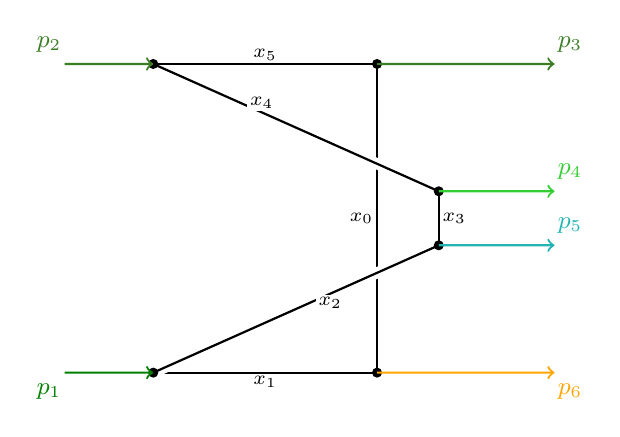
\begin{tikzpicture}[scale=.98]
 % The vertical placement displays the rapidity ordering
 % p3 >> (p4,p5) >> p6, while the top and bottom chains make the two
 % spacelike-collinear pairs manifest.
 \coordinate (v4) at (-2.20,2.00);
 \coordinate (v5) at ( .70,2.00);
 \coordinate (v3) at (1.50,.35);
 \coordinate (v2) at (1.50,-.35);
 \coordinate (v6) at ( .70,-2.00);
 \coordinate (v1) at (-2.20,-2.00);

 \draw[hrf internal] (v5)--node[hrf edge label,pos=.50,left] {$x_0$}(v6);
 \draw[hrf internal] (v6)--node[hrf edge label,pos=.50,below] {$x_1$}(v1);
 \draw[white,line width=4pt] (v1)--(v2);
 \draw[hrf internal] (v1)--node[hrf edge label,pos=.62,below] {$x_2$}(v2);
 \draw[hrf internal] (v2)--node[hrf edge label,pos=.50,right] {$x_3$}(v3);
 \draw[white,line width=4pt] (v3)--(v4);
 \draw[hrf internal] (v3)--node[hrf edge label,pos=.62,above] {$x_4$}(v4);
 \draw[hrf internal] (v4)--node[hrf edge label,pos=.50,above] {$x_5$}(v5);
 \foreach \v in {1,...,6} \node[hrf vertex] at (v\v) {};

 \draw[->,thick,OliveGreen] (-3.35,2.00)--(v4);
 \draw[->,thick,Green] (-3.35,-2.00)--(v1);
 \draw[->,thick,OliveGreen] (v5)--(3.00,2.00);
 \draw[->,thick,LimeGreen] (v3)--(3.00,.35);
 \draw[->,thick,TealBlue] (v2)--(3.00,-.35);
 \draw[->,thick,Orange] (v6)--(3.00,-2.00);
 \node[hrf leg label,text=OliveGreen] at (-3.55,2.25) {$p_2$};
 \node[hrf leg label,text=Green] at (-3.55,-2.25) {$p_1$};
 \node[hrf leg label,text=OliveGreen] at (3.20,2.25) {$p_3$};
 \node[hrf leg label,text=LimeGreen] at (3.20,.60) {$p_4$};
 \node[hrf leg label,text=TealBlue] at (3.20,-.10) {$p_5$};
 \node[hrf leg label,text=Orange] at (3.20,-2.25) {$p_6$};
\end{tikzpicture}
\caption{One-loop hexagon which displays a HR in both the (no recoil) NMRK and the DSC limits considered.
The nearly straight upper chain \(p_2\!-\!x_5\!-\!p_3\) and lower chain
\(p_1\!-\!x_1\!-\!p_6\) display the two spacelike-collinear pairs.  On the
right, the vertical separations display the rapidity ordering
\(p_3\gg(p_4,p_5)\gg p_6\); the relative order of \(p_4,p_5\) is immaterial
in NMRK.  The two crossings are deliberate and are not additional vertices.
This physical attachment ordering supports the HR (and associated Regge cut),
in contrast to the genuinely planar ordering \(123456\) with all four
emissions on one side.}
\label{fig:one-loop-hexagon}
\end{figure}

with \(\mathcal U=x_0+x_1+x_2+x_3+x_4+x_5\).  The full graph polynomial is
the same in both limits; only the invariant substitution changes.

In each case the cancelling monomials occur at different fixed-parameter
orders.  Thus \(\mathcal F_0\) does not contain the relevant cancellation
sector.  A face vector \(f\) first performs asymptotic-order alignment and
selects \(\mathcal F_\star=\mathcal F^{[f]}\).  Because
\(f\) and \(f+c\boldsymbol1\) select the same face, this discovery vector is
not yet the physical region vector.  The full occupied layer structure and
\(\mathcal U\) must fix the uniform component.

\subsubsection{Two-loop topology test and possible Regge-cut interpretation}

The two nearly horizontal chains in Fig.~\ref{fig:one-loop-hexagon} are the
\((23)\) and \((16)\) collinear sectors.  A \(t\)-channel exchange is an
internal path connecting these two chains.  The two central emissions
\(p_4,p_5\) may occur on the same such path or on two separate paths.
This distinction becomes explicit in the two-loop graphs used in the NMRK
and DSC audits.  With the external attachments of
Eq.~\eqref{eq:hexagon-edge-map}, their internal edges, in
\(x_0,\ldots,x_8\) order, are
\begin{align}
 E_{\rm PH}={}&\{(5,6),(1,8),(8,6),(1,2),(2,3),
                   (3,4),(4,7),(7,5),(7,8)\},\nonumber\\
 E_{\rm NPH}={}&\{(5,8),(1,8),(1,2),(2,3),(7,3),
                   (7,5),(4,7),(6,8),(4,6)\},\nonumber\\
 E_{\rm HP}={}&\{(5,6),(1,8),(8,6),(1,3),(3,4),
                   (4,7),(7,5),(7,2),(8,2)\}.
 \label{eq:two-loop-six-point-edges}
\end{align}

\begin{figure}[htbp]
\centering
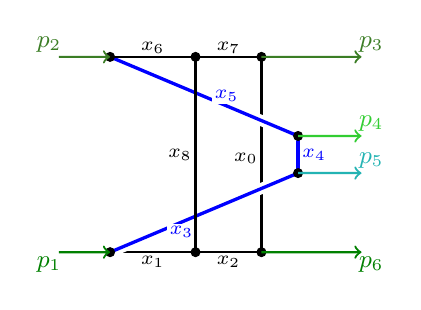
\begin{tikzpicture}[scale=.62]
 \coordinate (v4) at (-2.20,2.00);
 \coordinate (v7) at (-.45,2.00);
 \coordinate (v5) at ( .90,2.00);
 \coordinate (v3) at (1.65,.38);
 \coordinate (v2) at (1.65,-.38);
 \coordinate (v6) at ( .90,-2.00);
 \coordinate (v8) at (-.45,-2.00);
 \coordinate (v1) at (-2.20,-2.00);
 %\node[font=\small\bfseries] at (-.25,2.72) {planar hexbox};

 \draw[hrf internal] (v5)--node[hrf edge label,pos=.52,left] {$x_0$}(v6);
 \draw[hrf internal] (v1)--node[hrf edge label,pos=.50,below] {$x_1$}(v8);
 \draw[hrf internal] (v8)--node[hrf edge label,pos=.50,below] {$x_2$}(v6);
 \draw[white,line width=4pt] (v1)--(v2);
 \draw[hrf internal,very thick,blue] (v1)--
   node[hrf edge label,pos=.38,below,text=blue] {$x_3$}(v2);
 \draw[hrf internal,very thick,blue] (v2)--
   node[hrf edge label,pos=.50,right,text=blue] {$x_4$}(v3);
 \draw[white,line width=4pt] (v3)--(v4);
 \draw[hrf internal,very thick,blue] (v3)--
   node[hrf edge label,pos=.38,above,text=blue] {$x_5$}(v4);
 \draw[hrf internal] (v4)--node[hrf edge label,pos=.50,above] {$x_6$}(v7);
 \draw[hrf internal] (v7)--node[hrf edge label,pos=.50,above] {$x_7$}(v5);
 \draw[hrf internal] (v7)--node[hrf edge label,pos=.50,left] {$x_8$}(v8);
 \foreach \v in {1,...,8} \node[hrf vertex] at (v\v) {};
 \draw[->,thick,OliveGreen] (-3.25,2)--(v4);
 \draw[->,thick,Green] (-3.25,-2)--(v1);
 \draw[->,thick,OliveGreen] (v5)--(2.95,2);
 \draw[->,thick,LimeGreen] (v3)--(2.95,.38);
 \draw[->,thick,TealBlue] (v2)--(2.95,-.38);
 \draw[->,thick,Green] (v6)--(2.95,-2);
 \node[hrf leg label,text=OliveGreen] at (-3.45,2.25) {$p_2$};
 \node[hrf leg label,text=Green] at (-3.45,-2.25) {$p_1$};
 \node[hrf leg label,text=OliveGreen] at (3.15,2.25) {$p_3$};
 \node[hrf leg label,text=LimeGreen] at (3.15,.63) {$p_4$};
 \node[hrf leg label,text=TealBlue] at (3.15,-.13) {$p_5$};
 \node[hrf leg label,text=Green] at (3.15,-2.25) {$p_6$};
\end{tikzpicture}
\hspace{5mm}
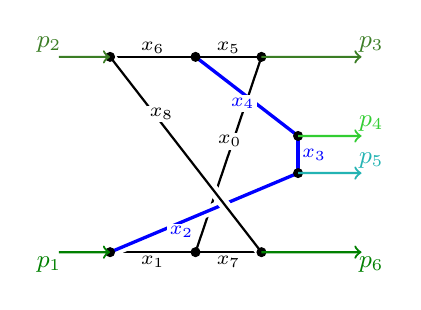
\begin{tikzpicture}[scale=.62]
 \coordinate (v4) at (-2.20,2.00);
 \coordinate (v7) at (-.45,2.00);
 \coordinate (v5) at ( .90,2.00);
 \coordinate (v3) at (1.65,.38);
 \coordinate (v2) at (1.65,-.38);
 \coordinate (v6) at ( .90,-2.00);
 \coordinate (v8) at (-.45,-2.00);
 \coordinate (v1) at (-2.20,-2.00);
 %\node[font=\small\bfseries] at (-.25,2.72) {nonplanar hexbox};

 \draw[hrf internal] (v5)--node[hrf edge label,pos=.48,above] {$x_0$}(v8);
 \draw[hrf internal] (v1)--node[hrf edge label,pos=.50,below] {$x_1$}(v8);
 \draw[white,line width=4pt] (v1)--(v2);
 \draw[hrf internal,very thick,blue] (v1)--
   node[hrf edge label,pos=.38,below,text=blue] {$x_2$}(v2);
 \draw[hrf internal,very thick,blue] (v2)--
   node[hrf edge label,pos=.50,right,text=blue] {$x_3$}(v3);
 \draw[hrf internal,very thick,blue] (v3)--
   node[hrf edge label,pos=.54,below,text=blue] {$x_4$}(v7);
 \draw[hrf internal] (v7)--node[hrf edge label,pos=.50,above] {$x_5$}(v5);
 \draw[hrf internal] (v4)--node[hrf edge label,pos=.50,above] {$x_6$}(v7);
 \draw[hrf internal] (v8)--node[hrf edge label,pos=.50,below] {$x_7$}(v6);
 \draw[white,line width=4pt] (v4)--(v6);
 \draw[hrf internal] (v4)--node[hrf edge label,pos=.34,above] {$x_8$}(v6);
 \foreach \v in {1,...,8} \node[hrf vertex] at (v\v) {};
 \draw[->,thick,OliveGreen] (-3.25,2)--(v4);
 \draw[->,thick,Green] (-3.25,-2)--(v1);
 \draw[->,thick,OliveGreen] (v5)--(2.95,2);
 \draw[->,thick,LimeGreen] (v3)--(2.95,.38);
 \draw[->,thick,TealBlue] (v2)--(2.95,-.38);
 \draw[->,thick,Green] (v6)--(2.95,-2);
 \node[hrf leg label,text=OliveGreen] at (-3.45,2.25) {$p_2$};
 \node[hrf leg label,text=Green] at (-3.45,-2.25) {$p_1$};
 \node[hrf leg label,text=OliveGreen] at (3.15,2.25) {$p_3$};
 \node[hrf leg label,text=LimeGreen] at (3.15,.63) {$p_4$};
 \node[hrf leg label,text=TealBlue] at (3.15,-.13) {$p_5$};
 \node[hrf leg label,text=Green] at (3.15,-2.25) {$p_6$};
\end{tikzpicture}

\vspace{3mm}
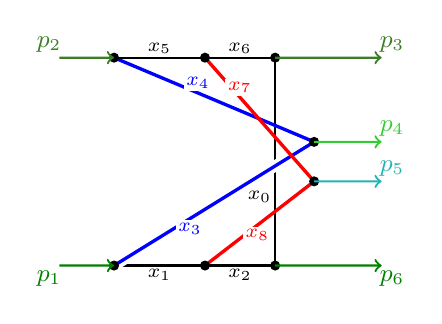
\begin{tikzpicture}[scale=.66]
 \coordinate (v4) at (-2.20,2.00);
 \coordinate (v7) at (-.45,2.00);
 \coordinate (v5) at ( .90,2.00);
 \coordinate (v3) at (1.65,.38);
 \coordinate (v2) at (1.65,-.38);
 \coordinate (v6) at ( .90,-2.00);
 \coordinate (v8) at (-.45,-2.00);
 \coordinate (v1) at (-2.20,-2.00);
 %\node[font=\small\bfseries] at (-.25,2.72) {hexagon--pentagon};

 \draw[hrf internal] (v5)--node[hrf edge label,pos=.67,left] {$x_0$}(v6);
 \draw[hrf internal] (v1)--node[hrf edge label,pos=.50,below] {$x_1$}(v8);
 \draw[hrf internal] (v8)--node[hrf edge label,pos=.50,below] {$x_2$}(v6);
 \draw[white,line width=4pt] (v1)--(v3);
 \draw[hrf internal,very thick,blue] (v1)--
   node[hrf edge label,pos=.38,below,text=blue] {$x_3$}(v3);
 \draw[hrf internal,very thick,blue] (v3)--
   node[hrf edge label,pos=.58,above,text=blue] {$x_4$}(v4);
 \draw[hrf internal] (v4)--node[hrf edge label,pos=.50,above] {$x_5$}(v7);
 \draw[hrf internal] (v7)--node[hrf edge label,pos=.50,above] {$x_6$}(v5);
 \draw[hrf internal,very thick,red] (v7)--
   node[hrf edge label,pos=.32,above,text=red] {$x_7$}(v2);
 \draw[hrf internal,very thick,red] (v2)--
   node[hrf edge label,pos=.52,below,text=red] {$x_8$}(v8);
 \foreach \v in {1,...,8} \node[hrf vertex] at (v\v) {};
 \draw[->,thick,OliveGreen] (-3.25,2)--(v4);
 \draw[->,thick,Green] (-3.25,-2)--(v1);
 \draw[->,thick,OliveGreen] (v5)--(2.95,2);
 \draw[->,thick,LimeGreen] (v3)--(2.95,.38);
 \draw[->,thick,TealBlue] (v2)--(2.95,-.38);
 \draw[->,thick,Green] (v6)--(2.95,-2);
 \node[hrf leg label,text=OliveGreen] at (-3.45,2.25) {$p_2$};
 \node[hrf leg label,text=Green] at (-3.45,-2.25) {$p_1$};
 \node[hrf leg label,text=OliveGreen] at (3.15,2.25) {$p_3$};
 \node[hrf leg label,text=LimeGreen] at (3.15,.63) {$p_4$};
 \node[hrf leg label,text=TealBlue] at (3.15,-.13) {$p_5$};
 \node[hrf leg label,text=Green] at (3.15,-2.25) {$p_6$};
\end{tikzpicture}
\caption{Two-loop graphs, drawn in the same rapidity-ordered embedding as Fig.~\ref{fig:one-loop-hexagon}.  In each graph the upper and lower horizontal chains are
the \((23)\) and \((16)\) collinear sectors.  The pair of diagrams at the top correspond to a planar and a nonplanar hexagonbox topologies in which both central emissions emerge from the same $t$-channel exchange (drawn in blue). The lower graph represents a hexagon-pentagon topology in which the two central emissions \(p_4\) and \(p_5\) emerges from separate $t$-channel exchange (blue and red). 
Vertices are denoted by black dots. The diagrams at the top, which feature the hexagon of Fig.~\ref{fig:one-loop-hexagon} as an externally labelled contraction minor have HRs, while the diagram at the bottom, which does not feature that hexagon as a contraction minor, does not.}
\label{fig:two-loop-six-point-graphs}
\end{figure}

The current certificates give
\begin{center}
\small
\begin{tabular}{@{}lccc@{}}
\toprule
Graph & central-emission paths & NMRK with \(w=z\) & generic DSC\\
\midrule
one-loop hexagon & same & 1 full certificate & 1 full certificate\\
planar hexbox & same & 4 full \(+\) 3 boundary & 1 full certificate\\
nonplanar hexbox & same & 1 full \(+\) 2 boundary & no certificate\\
hexagon--pentagon & separate & no staged candidate & no staged candidate\\
\bottomrule
\end{tabular}
\end{center}
These entries count certified vectors, not necessarily distinct physical
regions.  In the planar NMRK scan thirteen candidates reach the staged
alignment analysis, but six fail the restored-layer certification; the
seven entries in the table are those that survive the full native
\(\mathcal F\) audit.  Within the tested NMRK set, however, the same-exchange graphs have
an HR and the separate-exchange graph does not.  This is evidence for a
topology criterion, not yet a theorem; the DSC nonplanar-hexbox result also
shows that the topology is not sufficient in every kinematic expansion.

The crossed ordering is the six-point Mandelstam region in which Regge-cut
effects arise.  Bartels' reggeon calculus organized high-energy amplitudes
by one- and two-reggeon states in successive \(t\)-channels
\cite{Bartels:1980pe}.  Bartels, Lipatov and Sabio Vera later showed that, for
six and more legs, the BDS ansatz is incompatible with the Regge cuts
predicted by the BFKL approach in appropriate physical channels
\cite{Bartels:2008ce}, and computed the leading-logarithmic
color-octet cut contribution and the corresponding \(2\to4\) and \(3\to3\)
discontinuities \cite{Bartels:2008ce}.
That correction is the high-energy contribution that must reside in the
six-point BDS remainder function, and it initiated the extensive subsequent
study of remainder functions in multi-Regge kinematics.

It is therefore natural to conjecture that the HR found here is the
parameter-space origin of the relevant \(t\)-channel cut.  This connection
is not established by the present certificates alone.  It requires matching
the local positive pinch and its region integral to the appropriate
Mandelstam discontinuity and multi-reggeon exchange.  Enlarging the topology
sample in Fig.~\ref{fig:two-loop-six-point-graphs} is a direct way to test
the conjecture.

\subsubsection{NMRK with the additional surface \texorpdfstring{\(w=z\)}{w=z}}

Use the MSLCV chart
\begin{equation}
 X_{34}=\frac{\widehat X_{34}}{\eta},\qquad
 X_{56}=\frac{\widehat X_{56}}{\eta},\qquad
 X_{45},Q,z,\bar z,w,\bar w=O(1),\qquad \eta\to0^+,
 \label{eq:nmrk-scaling-example}
\end{equation}
with
\begin{equation}
 Q,\widehat X_{34},X_{45},\widehat X_{56},K_z>0,\qquad
 K_z=(1-z)(1-\bar z)>0.
 \label{eq:nmrk-domain-example}
\end{equation}
On this physical NMRK sheet \(z,\bar z\) and \(w,\bar w\) are conjugate
pairs.  The restriction \(w=z\), \(\bar w=\bar z\) is additional to NMRK.
For generic NMRK the relevant bilinear determinant is proportional to
\((w-z)(\bar w-\bar z)\), so the HR is absent.

On the restricted surface define
\begin{equation}
 L_1^N=(1+X_{45})x_4-\widehat X_{34}X_{45}x_5,\qquad
 L_2^N=(1+X_{45})x_2-K_zX_{45}\widehat X_{56}x_1.
 \label{eq:nmrk-factors-example}
\end{equation}
The selected face has
\begin{equation}
 \mathcal F_\star^N=\FSL^N+\FObs^N
 =\SLcolour{Q\widehat X_{34}\widehat X_{56}L_1^NL_2^N}+0.
 \label{eq:nmrk-decomposition-example}
\end{equation}
The two-stage vectors and certified answer are
\begin{align}
 \boldsymbol\phi_N&=(-1,-1,-2,-1,-2,-1),&
 \boldsymbol\rho_N&=(-1,-1,-1,-1,-1,-1),\nonumber\\
 \vHR^N&=(-2,-2,-3,-2,-3,-2;1),&
 (\WSL,\WHR)&=(-4,-3).
 \label{eq:nmrk-vector-example}
\end{align}
There is no intermediate cancellation layer.  At \(\WHR\),
\begin{align}
 \mathcal U_{-3}&=\HRcolour{x_2+x_4},\nonumber\\
 \mathcal F_{-3}&=\HRcolour{-Q\widehat X_{34}X_{45}\widehat X_{56}
 (K_zx_0x_2+K_zx_0x_4+\widehat X_{34}x_3x_5
 +K_z\widehat X_{56}x_1x_3)}.
 \label{eq:nmrk-WHR-example}
\end{align}
These monomials give a unique lower facet directly.  The required new
capability is asymptotic-order alignment itself; once the correct face is
exposed, the cancellation has depth one.  Restoring and testing every
native \(\eta\)-layer leaves this one-loop certificate unchanged.

\subsubsection{Generic double spacelike-collinear kinematics}

For DSC let \(\varepsilon\to0^+\) and use the real physical slice
\begin{equation}
 a<0,\qquad -1<\tau_1<0,\qquad \tau_2<-1,\qquad
 z_D<0,\qquad \bar z_D<0.
 \label{eq:dsc-domain-example}
\end{equation}
The symbols \(z_D,\bar z_D\) are conjugate on the standard real transverse
MRK branch, but after continuation to this DSC sheet they are two independent
real roots.  In the graph-polynomial sign convention the adjacent invariants
behave as
\begin{align}
 s_{12}&=-\frac{\tau_2}{a(1+\tau_1)(1+\tau_2)}+O(\varepsilon),&
 s_{23}&=\frac{\varepsilon^2\tau_1}{a\bar z_D}+O(\varepsilon^3),\nonumber\\
 s_{34}&=\frac{1}{(a-1)(1+\tau_2)}+O(\varepsilon),&
 s_{45}&=-\frac1a,\nonumber\\
 s_{56}&=\frac{\tau_1}{(a-1)(1+\tau_1)}+O(\varepsilon),&
 s_{16}&=\frac{\varepsilon^2\tau_2z_D}{a}+O(\varepsilon^3).
 \label{eq:dsc-invariants-example}
\end{align}
Thus \(s_{23},s_{16}<0\), while \(s_{12},s_{34},s_{45},s_{56}>0\), as
required for \(2\to4\) scattering with legs 1 and 2 incoming.

The cancellation factors and selected-face decomposition are
\begin{align}
 L_1^D&=(1+\tau_2)x_4+x_5,&
 L_2^D&=\tau_1x_1+(1+\tau_1)x_2,
 \label{eq:dsc-factors-example}\\
 \mathcal F_\star^D&=\FSL^D+\FObs^D
 =\SLcolour{-(a-1)a^2\bar z_D^{,2}L_1^DL_2^D}+0.
 \label{eq:dsc-decomposition-example}
\end{align}
Both factors have positive zeros,
\begin{equation}
 x_5=-(1+\tau_2)x_4>0,\qquad
 x_2=-\frac{\tau_1}{1+\tau_1}x_1>0.
 \label{eq:dsc-positive-pinch-example}
\end{equation}
For crossed double-timelike collinear splittings \(\tau_i>0\), so these
same factors have one sign for positive \(x_i\) and the pinch disappears.

The alignment vector and the provisional face-only HRF vector are
\begin{equation}
 \boldsymbol\phi_D=(-2,-2,-2,-1,-2,-2),\qquad
 \boldsymbol\rho_D^{(0)}=(-1,-1,-1,-1,-1,-1).
 \label{eq:dsc-discovery-vectors}
\end{equation}
The provisional vector is obtained from the isolated aligned face; it is not
the second vector in the final composition.  With
\(\ideal_D=\langle L_1^D,L_2^D\rangle\), the actual occupied layers obey
\begin{equation}
 \underbrace{\SLcolour{\mathcal F_{-4}\in\ideal_D^2}}_{
  \operatorname{ord}_{\ideal_D}=2}
 \; +\;
 \underbrace{\Othercolour{\mathcal F_{-3}\in\ideal_D\setminus\ideal_D^2}}_{
  \operatorname{ord}_{\ideal_D}=1}
 \; +\;
 \underbrace{\HRcolour{\mathcal F_{-2}\notin\ideal_D}}_{
  \operatorname{ord}_{\ideal_D}=0}.
 \label{eq:dsc-two-layer-colours}
\end{equation}
The middle layer contains 52 nonzero terms.  It is not a missing power of
\(\varepsilon\): it vanishes to first order on the common pinch.  The leading
\(\mathcal U\) layer is
\begin{equation}
 \mathcal U_{-2}=\HRcolour{x_0+x_1+x_2+x_4+x_5},
 \label{eq:dsc-U-leading}
\end{equation}
and the full ideal-jet balance gives
\begin{align}
 \boldsymbol\rho_D&=(0,0,0,1,0,0),&
 \boldsymbol\phi_D+\boldsymbol\rho_D
   &=(-2,-2,-2,0,-2,-2),\nonumber\\
 \vHR^D&=(-2,-2,-2,0,-2,-2;1),&
 (\WSL,\WHR)&=(-4,-2),
 \label{eq:dsc-vector-example}
\end{align}
with gap two.  A local dissection pulls back to this same vector.

This example is why asymptotic-order alignment cannot be treated as a
cosmetic preprocessing step.  HRF must (i) expose the cancelling face,
(ii) retain every occupied layer, (iii) compute successive ideal orders,
and (iv) use the first nonvanishing LP layer to fix the uniform ambiguity of
the face representative.  Simply adding
\(\boldsymbol\phi_D+\boldsymbol\rho_D^{(0)}\) would give the wrong total
vector and the wrong cancellation depth.  This is the concrete example for
the distinction between \(\boldsymbol\rho^{(0)}\) and the corrected
\(\boldsymbol\rho\) in Sec.~\ref{sec:alignment}.

\subsubsection{What the two limits share---and what they do not}

After their separate kinematic rescalings, the factor coefficients are
identified by
\begin{equation}
 \frac{K_zX_{45}\widehat X_{56}}{1+X_{45}}
 =-\frac{\tau_1}{1+\tau_1},
 \qquad
 \frac{\widehat X_{34}X_{45}}{1+X_{45}}
 =-\frac{1}{1+\tau_2}.
 \label{eq:composite-factor-map}
\end{equation}
Hence the two order-aligned \(\FSL\) supports describe the same type of
positive cancellation hypersurface.  The next layers differ:
\begin{center}
\begin{tabular}{@{}lccc@{}}
\toprule
Expansion & certified \(\boldsymbol v\) & \((\WSL,\WHR)\) & depth\\
\midrule
NMRK with \(w=z\) & \((-2,-2,-3,-2,-3,-2)\) & \((-4,-3)\) & 1\\
generic DSC & \((-2,-2,-2,0,-2,-2)\) & \((-4,-2)\) & 2\\
\bottomrule
\end{tabular}
\end{center}
The common generator does not make the two limits identical.  The first
resolved LP layer, and therefore the physical region vector, remembers the
path by which the singular hypersurface is approached.

\subsection*{What the examples teach}

\begin{center}
\small
\begin{tabular}{@{}>{\raggedright\arraybackslash}p{0.22\textwidth}
                    >{\raggedright\arraybackslash}p{0.26\textwidth}
                    >{\raggedright\arraybackslash}p{0.44\textwidth}@{}}
\toprule
Family & New structure & Capability needed not to miss the HR\\
\midrule
Crown & simultaneous positive cancellation, \(\FObs=0\) & keep a
multi-equation positive pinch and determine its uniform scaling\\
Crown descendants & contraction-minor boundary regions & scan boundary
strata and compare restricted ideals, not only parent interiors\\
Five-point seed & \(\FObs\ne0\), non-uniform scaling & isolate \(\FSL\)
before imposing the positive pinch; retain the obstruction\\
Vertex correction & primitive non-binomial factor & generate and test
general polynomial ideals rather than monomial pairs only\\
Five-point near-planar wide angle & three path normals and a
three-generator pair-product ideal & allow more than two polynomial
generators and certify the pullback from local coordinates\\
Five-point central-soft MRK & a two-factor cancellation exposed on a
nontrivial alignment face & preserve every native kinematic power when
composing the vectors; certify the resolved full-LP support\\
NMRK, \(w=z\) & cancellation on a nontrivial asymptotic face & align
orders before running the ordinary HRF construction\\
DSC & a second occupied cancellation layer & resolve the ideal filtration
and fix the uniform face ambiguity from the full LP polynomial\\
\bottomrule
\end{tabular}
\end{center}

The progression is cumulative.  Later examples require the earlier tests in
addition to their new feature.  In every case the final statement is again
geometric: after cancellation is resolved, the leading polynomial must be a
lower facet in coordinates adapted to the pinch.  HRF reconstructs the
coefficient and Landau information absent from the original Newton polytope;
it does not replace lower-facet certification.

Allowing massive internal propagators would relax the standing massless
multiaffinity assumption.  The resulting quadratic edge-parameter dependence
changes the possible cancellation jets and the local facet problem.  It is a
genuine extension of this framework, not another example in the present
tour.

\appendix
\section{Notation summary}

\begin{center}
\begin{tabular}{@{}p{0.38\textwidth}p{0.57\textwidth}@{}}
\toprule
Symbol & Meaning\\
\midrule
\(\delta\) & kinematic expansion parameter\\
\(\s\) & real kinematic coordinates; their physical domain \(\K\) is specified
  by explicit inequalities\\
\(x_e\) & independent LP edge parameter, integrated over \((0,\infty)\)\\
\(\mathcal C_{\rm LP}=\mathbb R_{>0}^{N}\) & non-projective LP integration
  contour\\
\(\mathcal P=\mathcal U+\mathcal F\) & Lee--Pomeransky polynomial\\
\(\deg_x\mathcal U=L,\ \deg_x\mathcal F=L+1\) & massless graph-polynomial
  degrees; both polynomials are linear in each individual \(x_e\)\\
\(\widehat{\mathcal P}=\mathcal F+x_0\mathcal U\) & optional homogeneous
  \((N+1)\)-parameter embedding\\
\(m_i=c_i(\s)\delta^{a_i}\x^{\boldsymbol r_i}\) & monomial of
  \(\mathcal P\)\\
\(\boldsymbol r_i\) & length-\(N\) LP-parameter exponent vector of \(m_i\)\\
\(\vec r_i=(\boldsymbol r_i;a_i)\) & augmented exponent point\\
\(\mathcal F_0\) & strict fixed-\(\x\) leading polynomial\\
\(\mathcal F^{[\phi]}\) & face selected by the preliminary alignment vector
  \(\boldsymbol\phi\)\\
\(x_e=\delta^{\phi_e}y_e\) & first transformation: asymptotic-order
  alignment\\
\(\mathcal F_\star\) & HRF starting polynomial, either
  \(\mathcal F_0\) or \(\mathcal F^{[\phi]}\)\\
\(\SSL\) & superleading monomial support selected by the scaling law\\
\(\FSL\) & superleading cancellation sector\\
\(\FObs\) & obstruction polynomial\\
\(f_j\) & non-monomial cancellation factor\\
\(\ideal\) & ideal of independent cancellation factors at the common pinch\\
\(\boldsymbol\rho^{(0)}\) & provisional face-only HRF scaling in the aligned
  variables\\
\(y_e=\delta^{\rho_e}z_e\) & corrected second-stage HRF scaling after all LP
  layers are restored\\
\(\boldsymbol v_{\HR}=\boldsymbol\phi+\boldsymbol\rho\) & composition of the
  two edge-parameter transformations\\
\(\vHR=(\boldsymbol v_{\HR};1)\) & certified total hidden-region vector; the
  last component is appended once and is not added stage by stage\\
\(\WSL\) & common individual weight of SL monomials\\
\(\WHR\) & first resolved nonvanishing LP weight after cancellation\\
\(\WHR-\WSL\) & cancellation depth\\
\SLcolour{red terms} & individually superleading sector at \(\WSL\)\\
\HRcolour{blue terms} & resolved physical leading layer at \(\WHR\)\\
\Othercolour{black terms} & all other layers, including intermediate
  ideal-valued cancellations\\
\bottomrule
\end{tabular}
\end{center}




\bibliographystyle{JHEP}
\bibliography{biblio}


\end{document}
